%=========================
% FrontMatter/appendices.tex
% Phụ lục chi tiết; tiếp tục bổ sung khi các chương còn lại được rút gọn.
%=========================

\clearpage
\appendix
\phantomsection
\section*{PHỤ LỤC}
\addcontentsline{toc}{section}{Phụ lục}

% Hai chương phân tích cũ được giữ làm tài liệu chi tiết. Nhãn và tham chiếu
% được thêm tiền tố để không trùng với các bảng, hình giữ lại ở Chương 2.
\begingroup
\let\AppendixOriginalLabel\label
\renewcommand{\label}[1]{\AppendixOriginalLabel{appendix:#1}}

% Mục A được đặt ngay sau tiêu đề PHỤ LỤC; các mục phụ lục tiếp theo
% vẫn dùng định dạng section thông thường và bắt đầu ở trang mới.
\titleformat{\section}
  {\Large\bfseries\color{HCMUTDarkBlue}}
  {Chương~\thesection}{0.8em}{--\ }
%=========================
% Appendices/02-PhanTichYeuCau-ChiTietYeuCau.tex
% Phụ lục A – Yêu cầu chức năng chi tiết
%=========================
\section{Yêu cầu chức năng chi tiết}

Phụ lục này trình bày danh mục yêu cầu chức năng của trợ lý mua sắm đa phương
thức và website thương mại điện tử. Yêu cầu dữ liệu và yêu cầu phi chức năng đã
được trình bày đầy đủ trong Chương 2 nên không lặp lại tại đây.

\subsection{Trợ lý mua sắm đa phương thức}

\begin{longtable}{|p{0.12\linewidth}|p{0.25\linewidth}|p{0.45\linewidth}|p{0.10\linewidth}|}
\caption{Yêu cầu chức năng AI}\label{tab:ai-functional-requirements}\\
\hline
\textbf{Mã} & \textbf{Chức năng} & \textbf{Mô tả} & \textbf{Ưu tiên} \\
\hline
\endfirsthead
\hline
\textbf{Mã} & \textbf{Chức năng} & \textbf{Mô tả} & \textbf{Ưu tiên} \\
\hline
\endhead
FR-AI-01 & Tìm kiếm text & Tạo text embedding và truy hồi sản phẩm phù hợp theo ngữ nghĩa. & Cao \\
\hline
FR-AI-02 & Tìm kiếm image & Nhận ảnh, tạo image embedding và tìm sản phẩm tương tự. & Cao \\
\hline
FR-AI-03 & Hybrid search & Kết hợp ảnh tham chiếu với điều kiện văn bản. & Cao \\
\hline
FR-AI-04 & Phân tích truy vấn & Trích xuất loại sản phẩm, màu, kích thước, thương hiệu và khoảng giá. & Cao \\
\hline
FR-AI-05 & Lọc metadata & Lọc theo giá, danh mục, màu sắc, thương hiệu và tồn kho. & Cao \\
\hline
FR-AI-06 & Hội thoại nhiều lượt & Duy trì ngữ cảnh, ràng buộc và lựa chọn trước đó. & Cao \\
\hline
FR-AI-07 & Phản hồi có căn cứ & Chỉ sinh phản hồi từ dữ liệu sản phẩm được truy hồi. & Cao \\
\hline
FR-AI-08 & Fusion và rerank & Hợp nhất các nhánh text/image và sắp xếp ứng viên. & Cao \\
\hline
FR-AI-09 & Gợi ý tương tự & Đề xuất sản phẩm liên quan dựa trên độ tương đồng. & TB \\
\hline
FR-AI-10 & Đồng bộ chỉ mục & Cập nhật hoặc xóa embedding/payload Qdrant khi sản phẩm thay đổi. & Cao \\
\hline
FR-AI-11 & Lịch sử và log & Lưu checkpoint, trạng thái phiên, latency và log cần thiết. & TB \\
\hline
FR-AI-12 & Phản hồi dự phòng & thương mại điện tử cơ bản vẫn hoạt động khi dịch vụ AI tạm lỗi. & Cao \\
\hline
\end{longtable}
YOLO chỉ là bước crop tùy chọn ở môi trường phát triển; tìm kiếm đa ngôn ngữ và mô hình local là hướng mở rộng.

\subsection{Website thương mại điện tử}

\begin{longtable}{|p{0.14\linewidth}|p{0.26\linewidth}|p{0.42\linewidth}|p{0.10\linewidth}|}
\caption{Yêu cầu chức năng thương mại điện tử}\label{tab:ecommerce-functional-requirements}\\
\hline
\textbf{Mã} & \textbf{Chức năng} & \textbf{Mô tả} & \textbf{Ưu tiên} \\
\hline
\endfirsthead
\hline
\textbf{Mã} & \textbf{Chức năng} & \textbf{Mô tả} & \textbf{Ưu tiên} \\
\hline
\endhead
EC-FR-01 & Tài khoản & Đăng ký, đăng nhập, cập nhật thông tin và đổi mật khẩu. & Cao \\
\hline
EC-FR-02 & Sản phẩm/giỏ hàng & Xem, lọc sản phẩm; thêm, sửa, xóa sản phẩm trong giỏ. & Cao \\
\hline
EC-FR-03 & Đặt hàng COD & Xác nhận nhận hàng, tạo đơn và thanh toán khi nhận hàng. & Cao \\
\hline
EC-FR-04 & Đơn hàng/đánh giá & Theo dõi đơn hàng và đánh giá sản phẩm đã mua. & TB \\
\hline
EC-FR-05 & Quản trị & Quản lý sản phẩm, ảnh, tồn kho, đơn hàng, người dùng, blog và dashboard. & Cao \\
\hline
\end{longtable}


\titleformat{\section}
  {\clearpage\Large\bfseries\color{HCMUTDarkBlue}}
  {Chương~\thesection}{0.8em}{--\ }
%=========================
% Appendices/02-PhanTichYeuCau-ChiTietMoHinh.tex
% Phụ lục B – Mô hình phân tích chi tiết
%=========================
\section{Mô hình phân tích chi tiết}

Phụ lục này bổ sung các sơ đồ quy trình nghiệp vụ, một bảng tổng hợp đặc tả
Usecase và các sơ đồ hoạt động không xuất hiện trong Chương 2.
\subsection{Quy trình nghiệp vụ}
\par\medskip\noindent
\begin{minipage}{\textwidth}
\subsubsection{Quy trình thương mại điện tử tổng quát}

Quy trình thương mại điện tử tổng quát mô tả luồng mua sắm cơ bản của người dùng trên website, từ khi truy cập hệ thống, tìm kiếm sản phẩm, thêm vào giỏ hàng, đặt hàng, thanh toán cho đến theo dõi và đánh giá đơn hàng. Bên cạnh đó, quản trị viên tham gia vào quy trình thông qua việc xử lý và cập nhật trạng thái đơn hàng.


\centering
\resizebox{0.58\textwidth}{!}{
\begin{tikzpicture}[node distance=0.8cm, >=stealth]

\tikzstyle{activity} = [
    rectangle,
    rounded corners,
    draw,
    align=center,
    minimum width=4.1cm,
    minimum height=0.8cm
]

\tikzstyle{decision} = [
    diamond,
    draw,
    align=center,
    aspect=2,
    inner sep=1pt
]

%================ NODES =================
\node[activity, fill=blue!10] (start) {Người dùng truy cập website};

\node[activity, fill=green!10, below=of start] (login) {Đăng ký / Đăng nhập};

\node[activity, fill=orange!15, right=2.2cm of login] (account) {Quản lý tài khoản};

\node[activity, fill=green!10, below=of login] (info) {Xem trang chủ / blog / chính sách};

\node[activity, fill=orange!15, right=2.2cm of info] (support) {Liên hệ / Chatbot hỗ trợ};

\node[activity, fill=green!10, below=of info] (browse) {Xem và tìm kiếm sản phẩm};

\node[activity, fill=green!10, below=of browse] (detail) {Xem chi tiết sản phẩm};

\node[decision, fill=yellow!15, below=1cm of detail] (buy) {Mua sản phẩm?};

\node[activity, fill=green!10, below=1cm of buy] (cart) {Thêm vào giỏ hàng};

\node[activity, fill=green!10, below=of cart] (checkout) {Kiểm tra giỏ hàng};

\node[activity, fill=green!10, below=of checkout] (shipping) {Nhập thông tin giao hàng};

\node[activity, fill=green!10, below=of shipping] (payment) {Chọn phương thức thanh toán};

\node[activity, fill=green!10, below=of payment] (order) {Tạo đơn hàng};

\node[activity, fill=orange!15, right=2.6cm of order] (adminorder) {Admin quản lý và cập nhật\\trạng thái đơn hàng};

\node[activity, fill=orange!15, above=of adminorder] (admindata) {Admin quản lý sản phẩm / blog /\\người dùng};

\node[activity, fill=orange!15, above=of admindata] (admindash) {Admin đăng nhập /\\Xem dashboard};

\node[activity, fill=green!10, below=of order] (track) {Theo dõi / xem lịch sử đơn hàng};

\node[decision, fill=yellow!15, below=1cm of track] (done) {Đơn hàng\\hoàn tất?};

\node[activity, fill=green!10, below=1cm of done] (review) {Đánh giá sản phẩm};

\node[activity, fill=blue!10, below=of review] (end) {Kết thúc};

%================ MAIN USER FLOW =================
\draw[->, thick] (start) -- (login);
\draw[->, thick] (login) -- (info);
\draw[->, thick] (info) -- (browse);
\draw[->, thick] (browse) -- (detail);
\draw[->, thick] (detail) -- (buy);

\draw[->, thick] (buy) -- node[right]{Có} (cart);
\draw[->, thick] (buy.west) -- ++(-1.6,0) node[left]{Không} |- (browse.west);

\draw[->, thick] (cart) -- (checkout);
\draw[->, thick] (checkout) -- (shipping);
\draw[->, thick] (shipping) -- (payment);
\draw[->, thick] (payment) -- (order);

\draw[->, thick] (order) -- (track);
\draw[->, thick] (track) -- (done);

\draw[->, thick] (done) -- node[right]{Có} (review);
\draw[->, thick] (done.west) -- ++(-1.6,0) node[left]{Chưa} |- (track.west);

\draw[->, thick] (review) -- (end);

%================ USER SIDE FLOWS =================
\draw[->, thick] (login.east) -- (account.west);
\draw[->, thick] (info.east) -- (support.west);

%================ ADMIN FLOW =================
\draw[->, thick] (admindash) -- (admindata);
\draw[->, thick] (admindata) -- (adminorder);

% Admin tham gia sau khi đơn hàng được tạo
\draw[->, thick] (order.east) -- (adminorder.west);

% Sau khi admin cập nhật, người dùng theo dõi trạng thái
\draw[->, thick] (adminorder.south) |- (track.east);

\end{tikzpicture}
}
\captionof{figure}{Quy trình thương mại điện tử tổng quát}
\label{fig:ecommerce-process}
\end{minipage}
\par\medskip

\par\medskip\noindent
\begin{minipage}{\textwidth}
\subsubsection{Quy trình AI Shopping Assistant tổng quát}

Quy trình AI Shopping Assistant mô tả luồng xử lý có kiểm soát từ lúc nhận truy vấn đến khi trả kết quả. Sau khi đọc memory và phân tích ý định, hệ thống tạo embedding, truy hồi song song từ collection text/image của Qdrant, lọc metadata, fusion, rerank, lấy thông tin hiện hành từ MySQL và mới sử dụng LLM để sinh phản hồi có căn cứ. Khi không có kết quả hoặc dịch vụ AI lỗi, hệ thống ghi log, thông báo phù hợp và giữ các chức năng thương mại điện tử cơ bản hoạt động.


\centering

\begin{tikzpicture}

%================ BOXES =================
\draw[rounded corners, fill=blue!10]
(0,0) rectangle (4,1)
node[pos=.5]{Người dùng};

\draw[rounded corners, fill=green!10]
(0,-2) rectangle (4,-1)
node[pos=.5]{Gửi truy vấn};

\draw[rounded corners, fill=green!10]
(0,-4) rectangle (4,-3)
node[pos=.5]{Query Understanding};

\draw[rounded corners, fill=purple!10]
(0,-6) rectangle (4,-5)
node[pos=.5]{Multimodal Embedding};

\draw[rounded corners, fill=orange!15]
(6,-6) rectangle (9,-5)
node[pos=.5]{Qdrant Search};

\draw[rounded corners, fill=green!10]
(0,-8) rectangle (4,-7)
node[pos=.5]{Metadata + Fusion};

\draw[rounded corners, fill=green!10]
(0,-10) rectangle (4,-9)
node[pos=.5]{Managed Reranking};

\draw[rounded corners, fill=purple!10]
(0,-12) rectangle (4,-11)
node[pos=.5]{Grounded Response};

\draw[rounded corners, fill=orange!15]
(6,-12) rectangle (9,-11)
node[pos=.5]{Memory};

\draw[rounded corners, fill=green!10]
(0,-14) rectangle (4,-13)
node[pos=.5]{Result / Fallback};

%================ ARROWS =================
\draw[->, thick] (2,0) -- (2,-1);

\draw[->, thick] (2,-2) -- (2,-3);

\draw[->, thick] (2,-4) -- (2,-5);

\draw[->, thick] (2,-6) -- (2,-7);

\draw[->, thick] (2,-8) -- (2,-9);

\draw[->, thick] (2,-10) -- (2,-11);

\draw[->, thick] (2,-12) -- (2,-13);

%================ DB FLOW =================
\draw[->, thick] (4,-5.5) -- (6,-5.5);

\draw[->, thick] (7.5,-6) -- (7.5,-7.5) -- (4,-7.5);

%================ MEMORY =================
\draw[->, thick] (4,-11.5) -- (6,-11.5);

\draw[->, thick] (7.5,-11) -- (7.5,-10) -- (4,-10);

\end{tikzpicture}

\captionof{figure}{Quy trình nghiệp vụ hệ thống AI Shopping Assistant}
\label{fig:business-process}
\end{minipage}
\par\medskip


%=====================================================
\par\medskip\noindent
\begin{minipage}{\textwidth}
\subsubsection{Tìm kiếm bằng văn bản}

Đây là quy trình cốt lõi trong hệ thống AI Shopping Assistant. Người dùng nhập truy vấn bằng ngôn ngữ tự nhiên thay vì keyword đơn giản. Hệ thống sẽ thực hiện semantic embedding và vector retrieval để tìm các sản phẩm phù hợp về mặt ngữ nghĩa.

% \textbf{Luồng xử lý chính:}

% \begin{enumerate}
%     \item Người dùng nhập truy vấn văn bản.
%     \item Query processing module thực hiện normalize và query understanding.
%     \item Text embedding model sinh vector embedding cho truy vấn.
%     \item Vector database thực hiện ANN search.
%     \item Hệ thống rerank top-k candidate.
%     \item Trả về danh sách sản phẩm phù hợp.
% \end{enumerate}

% \textbf{Diagram cần thiết kế:}
% \begin{itemize}
%     \item Activity Diagram cho Semantic Search
%     \item Data Flow Diagram cho text retrieval pipeline
% \end{itemize}

\centering

\begin{tikzpicture}

%================ BOXES =================
\draw[rounded corners, fill=blue!10]
(0,0) rectangle (4,1)
node[pos=.5]{Người dùng};

\draw[rounded corners, fill=green!10]
(0,-2) rectangle (4,-1)
node[pos=.5]{Nhập text query};

\draw[rounded corners, fill=green!10]
(0,-4) rectangle (4,-3)
node[pos=.5]{Query Understanding};

\draw[rounded corners, fill=purple!10]
(0,-6) rectangle (4,-5)
node[pos=.5]{Text Embedding};

\draw[rounded corners, fill=orange!15]
(6,-6) rectangle (9,-5)
node[pos=.5]{Qdrant Text};

\draw[rounded corners, fill=green!10]
(0,-8) rectangle (4,-7)
node[pos=.5]{ANN Search};

\draw[rounded corners, fill=green!10]
(0,-10) rectangle (4,-9)
node[pos=.5]{Metadata + Rerank};

\draw[rounded corners, fill=green!10]
(0,-12) rectangle (4,-11)
node[pos=.5]{MySQL + Results};

%================ ARROWS =================
\draw[->, thick] (2,0) -- (2,-1);
\draw[->, thick] (2,-2) -- (2,-3);
\draw[->, thick] (2,-4) -- (2,-5);
\draw[->, thick] (2,-6) -- (2,-7);
\draw[->, thick] (2,-8) -- (2,-9);
\draw[->, thick] (2,-10) -- (2,-11);

%================ VECTOR DB =================
\draw[->, thick] (4,-5.5) -- (6,-5.5);

\draw[->, thick]
(7.5,-6) -- (7.5,-7.5) -- (4,-7.5);

\end{tikzpicture}

\captionof{figure}{Quy trình tìm kiếm sản phẩm bằng văn bản}
\label{fig:text-search-process}
\end{minipage}
\par\medskip


%=====================================================
\par\medskip\noindent
\begin{minipage}{\textwidth}
\subsubsection{Tìm kiếm bằng hình ảnh}

Hệ thống hỗ trợ image retrieval nhằm cho phép người dùng tải lên hình ảnh sản phẩm và tìm các sản phẩm tương tự trong cơ sở dữ liệu.

Hệ thống kiểm tra định dạng và tiền xử lý ảnh trước khi tạo image embedding. YOLO chỉ là bước crop tùy chọn ở môi trường phát triển; khi production tắt YOLO, ảnh gốc được sử dụng trực tiếp. Sau đó hệ thống truy hồi image collection, lọc metadata nếu có điều kiện bổ sung và rerank kết quả.

% \textbf{Luồng xử lý chính:}

% \begin{enumerate}
%     \item Người dùng upload hình ảnh.
%     \item Hệ thống kiểm tra định dạng và preprocess ảnh.
%     \item YOLO model phát hiện và crop đối tượng sản phẩm.
%     \item Image embedding model sinh vector embedding.
%     \item Vector database thực hiện similarity search.
%     \item Trả về các sản phẩm tương tự.
% \end{enumerate}

% \textbf{Diagram cần thiết kế:}
% \begin{itemize}
%     \item Activity Diagram cho Image Retrieval
%     \item AI Pipeline Diagram cho YOLO + CLIP/SigLIP
% \end{itemize}


\centering

\begin{tikzpicture}

\draw[rounded corners, fill=blue!10]
(0,0) rectangle (4,1)
node[pos=.5]{Người dùng};

\draw[rounded corners, fill=green!10]
(0,-2) rectangle (4,-1)
node[pos=.5]{Upload hình ảnh};

\draw[rounded corners, fill=green!10]
(0,-4) rectangle (4,-3)
node[pos=.5]{Validate Image};

\draw[rounded corners, fill=purple!10]
(0,-6) rectangle (4,-5)
node[pos=.5]{Optional YOLO};

\draw[rounded corners, fill=purple!10]
(0,-8) rectangle (4,-7)
node[pos=.5]{Image Embedding};

\draw[rounded corners, fill=orange!15]
(6,-8) rectangle (9,-7)
node[pos=.5]{Qdrant Image};

\draw[rounded corners, fill=green!10]
(0,-10) rectangle (4,-9)
node[pos=.5]{Metadata + Rerank};

\draw[rounded corners, fill=green!10]
(0,-12) rectangle (4,-11)
node[pos=.5]{Results / Fallback};

%================ ARROWS =================
\draw[->, thick] (2,0) -- (2,-1);
\draw[->, thick] (2,-2) -- (2,-3);
\draw[->, thick] (2,-4) -- (2,-5);
\draw[->, thick] (2,-6) -- (2,-7);
\draw[->, thick] (2,-8) -- (2,-9);
\draw[->, thick] (2,-10) -- (2,-11);

%================ DB =================
\draw[->, thick] (4,-7.5) -- (6,-7.5);

\draw[->, thick]
(7.5,-8) -- (7.5,-9.5) -- (4,-9.5);

\end{tikzpicture}

\captionof{figure}{Quy trình tìm kiếm bằng hình ảnh}
\label{fig:image-search-process}
\end{minipage}
\par\medskip



%=====================================================
\par\medskip\noindent
\begin{minipage}{\textwidth}
\subsubsection{Tìm kiếm kết hợp ảnh--văn bản}

Hybrid Search sử dụng chính sách image-conditioned: ảnh tham chiếu xác định độ tương tự
trực quan, còn văn bản được tách thành các ràng buộc tìm kiếm. Hệ thống truy hồi ứng
viên theo ảnh và chỉ dùng truy hồi văn bản để phục hồi khi số ứng viên hợp lệ chưa đủ
hoặc độ tương tự ảnh còn thấp.

Ví dụ:
\begin{quote}
“Tìm áo giống hình này nhưng màu đen”
\end{quote}

Trong trường hợp này, hình ảnh giữ đặc trưng của sản phẩm tham chiếu, còn yêu cầu
``màu đen'' trở thành ràng buộc bắt buộc khi lọc ứng viên.

% \textbf{Luồng xử lý chính:}

% \begin{enumerate}
%     \item Người dùng nhập text query và upload image.
%     \item Hệ thống sinh text embedding và image embedding.
%     \item Fusion module kết hợp hai vector embedding.
%     \item Vector database thực hiện hybrid retrieval.
%     \item Reranker tối ưu kết quả cuối cùng.
% \end{enumerate}

% \textbf{Diagram cần thiết kế:}
% \begin{itemize}
%     \item Activity Diagram cho Hybrid Search
%     \item Multimodal Fusion Diagram
% \end{itemize}


\centering

\begin{tikzpicture}[
    font=\small,
    >=Stealth,
    process/.style={
        draw,
        rounded corners,
        minimum height=0.82cm,
        text width=4.7cm,
        align=center,
        fill=green!10
    },
    embedding/.style={process, fill=purple!10},
    storage/.style={process, fill=orange!15},
    decision/.style={
        diamond,
        draw,
        aspect=2.5,
        text width=3.1cm,
        align=center,
        inner sep=1pt,
        fill=yellow!12
    },
    flow/.style={->, thick}
]

\node[process, fill=blue!10] (input) {Văn bản + ảnh};
\node[process, below=0.42cm of input] (intent) {Tách ràng buộc văn bản};
\node[embedding, below=0.42cm of intent] (image-embedding) {Tạo Image Embedding};
\node[storage, below=0.42cm of image-embedding] (image-retrieval)
    {Truy hồi ứng viên ảnh};
\node[process, below=0.42cm of image-retrieval] (constraint-check)
    {Kiểm tra ràng buộc};
\node[decision, below=0.58cm of constraint-check] (enough)
    {Ứng viên ảnh đạt yêu cầu?};

\node[embedding, right=1.65cm of enough] (text-embedding)
    {Tạo Text Embedding};
\node[storage, below=0.42cm of text-embedding] (text-retrieval)
    {Truy hồi ứng viên văn bản};
\node[process, below=0.42cm of text-retrieval] (recovery)
    {Bổ sung ứng viên hợp lệ};

\node[process, below=1.05cm of enough] (ranking)
    {Xếp hạng theo ảnh};
\node[process, below=0.42cm of ranking] (top-k)
    {Kiểm tra và lấy Top-K};
\node[process, fill=blue!10, below=0.42cm of top-k] (response)
    {Trả danh sách sản phẩm};

\draw[flow] (input) -- (intent);
\draw[flow] (intent) -- (image-embedding);
\draw[flow] (image-embedding) -- (image-retrieval);
\draw[flow] (image-retrieval) -- (constraint-check);
\draw[flow] (constraint-check) -- (enough);
\draw[flow] (enough) -- node[left]{Có} (ranking);
\draw[flow] (enough.east) -- node[above]{Không} (text-embedding.west);
\draw[flow] (text-embedding) -- (text-retrieval);
\draw[flow] (text-retrieval) -- (recovery);
\draw[flow] (recovery.west) -| (ranking.east);
\draw[flow] (ranking) -- (top-k);
\draw[flow] (top-k) -- (response);

\end{tikzpicture}

\captionof{figure}{Quy trình Hybrid Search theo chính sách image-conditioned}
\label{fig:hybrid-search-process}
\end{minipage}
\par\medskip



%=====================================================
\FloatBarrier

\subsection{Tổng hợp đặc tả Usecase}

Ba sơ đồ Usecase tổng quan đã được trình bày tại Chương 2. Bảng dưới đây tổng hợp
tác nhân, mục tiêu và điều kiện hoặc kết quả chính của các Usecase; báo cáo không
tách thành bảng đặc tả riêng cho từng Usecase.

\small
\begin{longtable}{|p{0.10\textwidth}|p{0.20\textwidth}|p{0.15\textwidth}|p{0.22\textwidth}|p{0.22\textwidth}|}
    \caption{Tổng hợp đặc tả Usecase}\label{appendix:tab:usecase-summary}\\
    \hline
    \textbf{Mã} & \textbf{Usecase} & \textbf{Tác nhân} & \textbf{Mục tiêu} & \textbf{Điều kiện/Kết quả chính} \\ \hline
    \endfirsthead
    \hline
    \textbf{Mã} & \textbf{Usecase} & \textbf{Tác nhân} & \textbf{Mục tiêu} & \textbf{Điều kiện/Kết quả chính} \\ \hline
    \endhead
    UC-KH-01 & Đăng ký & Khách vãng lai & Tạo tài khoản & Thông tin hợp lệ; tài khoản được tạo. \\ \hline
    UC-KH-02 & Đăng nhập & Khách vãng lai & Truy cập chức năng cá nhân & Thông tin đúng; phiên đăng nhập được thiết lập. \\ \hline
    UC-KH-03 & Khôi phục mật khẩu & Khách vãng lai & Cấp lại quyền truy cập & Email tồn tại; mật khẩu được đặt lại an toàn. \\ \hline
    UC-KH-04 & Xem danh mục & Người dùng & Duyệt nhóm sản phẩm & Danh mục khả dụng; danh sách được hiển thị. \\ \hline
    UC-KH-05 & Tìm kiếm truyền thống & Người dùng & Tìm theo từ khóa và bộ lọc & Truy vấn hợp lệ; trả sản phẩm phù hợp. \\ \hline
    UC-KH-06 & Xem chi tiết sản phẩm & Người dùng & Xem giá, biến thể và tồn kho & Sản phẩm hoạt động; dữ liệu hiện hành được hiển thị. \\ \hline
    UC-KH-07 & So sánh sản phẩm & Người dùng & Đối chiếu thuộc tính & Có sản phẩm hợp lệ; bảng so sánh được tạo. \\ \hline
    UC-KH-08 & Xem bài viết & Người dùng & Tra cứu nội dung tư vấn & Bài viết đã xuất bản; nội dung được hiển thị. \\ \hline
    UC-KH-09 & Quản lý hồ sơ & Khách hàng & Cập nhật thông tin cá nhân & Đã đăng nhập; dữ liệu được lưu đúng chủ sở hữu. \\ \hline
    UC-KH-10 & Quản lý giỏ hàng & Khách hàng & Thêm, sửa hoặc xóa sản phẩm & Biến thể hợp lệ; giỏ phản ánh giá và tồn kho hiện hành. \\ \hline
    UC-KH-11 & Đặt hàng COD & Khách hàng & Tạo đơn thanh toán khi nhận hàng & Giỏ và địa chỉ hợp lệ; đơn COD được tạo. \\ \hline
    UC-KH-12 & Xem lịch sử đơn hàng & Khách hàng & Theo dõi đơn đã đặt & Chỉ hiển thị đơn thuộc khách hàng. \\ \hline
    UC-KH-13 & Hủy đơn hàng & Khách hàng & Hủy đơn còn cho phép & Đơn đúng chủ và trạng thái; tồn kho được hoàn trả. \\ \hline
    UC-KH-14 & Xác nhận nhận hàng & Khách hàng & Hoàn tất đơn đã giao & Đơn đang giao; trạng thái chuyển hoàn tất. \\ \hline
    UC-KH-15 & Đánh giá sản phẩm & Khách hàng & Gửi nhận xét sau mua & Đơn hoàn tất; đánh giá được ghi nhận. \\ \hline
    UC-KH-16 & Sử dụng trợ lý AI & Người dùng & Truy cập chức năng AI & Yêu cầu hợp lệ; chuyển đến Usecase AI tương ứng. \\ \hline
    UC-AD-01 & Xem dashboard & Quản trị viên & Theo dõi vận hành & Có quyền truy cập; số liệu được hiển thị. \\ \hline
    UC-AD-02 & Quản lý khách hàng & Quản trị viên & Quản lý tài khoản & Có quyền; thay đổi được lưu và ghi nhận. \\ \hline
    UC-AD-03 & Quản lý danh mục & Quản trị viên & Tổ chức danh mục & Dữ liệu hợp lệ; cấu trúc được cập nhật. \\ \hline
    UC-AD-04 & Quản lý sản phẩm & Quản trị viên & Quản lý sản phẩm và biến thể & Dữ liệu được lưu và đánh dấu đồng bộ AI. \\ \hline
    UC-AD-05 & Điều chỉnh tồn kho & Quản trị viên & Cập nhật số lượng bán & Biến thể tồn tại; tồn kho và lịch sử được cập nhật. \\ \hline
    UC-AD-06 & Quản lý đơn hàng & Quản trị viên & Xử lý vòng đời đơn & Trạng thái tuân thủ quy tắc chuyển đổi. \\ \hline
    UC-AD-07 & Xác nhận đơn COD & Quản trị viên & Tiếp nhận đơn COD & Đơn và tồn kho hợp lệ; giao dịch được ghi nhận. \\ \hline
    UC-AD-08 & Quản lý bài viết & Quản trị viên & Soạn và xuất bản nội dung & Nội dung hợp lệ; trạng thái được cập nhật. \\ \hline
    UC-AD-09 & Quản lý khuyến mãi & Quản trị viên & Cấu hình giảm giá & Điều kiện và thời gian hợp lệ; chương trình được lưu. \\ \hline
    UC-AD-10 & Kiểm duyệt đánh giá & Quản trị viên & Duyệt hoặc ẩn phản hồi & Có quyền; trạng thái đánh giá được cập nhật. \\ \hline
    UC-AI-01 & Tìm kiếm văn bản & Người dùng & Tìm theo ngữ nghĩa & Truy vấn hợp lệ; trả danh sách đã xếp hạng. \\ \hline
    UC-AI-02 & Tìm kiếm hình ảnh & Người dùng & Tìm sản phẩm tương tự & Ảnh hợp lệ; trả kết quả tương tự. \\ \hline
    UC-AI-03 & Tìm kiếm kết hợp & Người dùng & Kết hợp văn bản và ảnh & Có đầu vào hợp lệ; kết quả được hợp nhất và xếp hạng. \\ \hline
    UC-AI-04 & Chat tư vấn đa lượt & Người dùng & Nhận tư vấn theo ngữ cảnh & Phiên hợp lệ; phản hồi và ngữ cảnh được lưu. \\ \hline
    UC-AI-05 & Chọn vùng ảnh & Người dùng & Giới hạn đối tượng cần tìm & Vùng chọn hợp lệ; chuyển sang tìm kiếm ảnh hoặc kết hợp. \\ \hline
    UC-AI-06 & Gửi phản hồi AI & Khách hàng & Đánh giá mức hữu ích & Có kết quả; phản hồi được lưu. \\ \hline
    UC-AI-07 & Đồng bộ chỉ mục & Quản trị viên & Cập nhật vector sản phẩm & Có quyền; tác vụ đồng bộ được thực thi. \\ \hline
    UC-AI-08 & Theo dõi đồng bộ & Quản trị viên & Theo dõi tiến độ và lỗi & Có mã tác vụ; trạng thái được hiển thị. \\ \hline
    UC-AI-09 & Kiểm tra embedding & Quản trị viên & Phát hiện sai lệch chỉ mục & Chỉ mục truy cập được; báo cáo được tạo. \\ \hline
\end{longtable}
\normalsize

\FloatBarrier

\subsection{Các sơ đồ hoạt động bổ sung}

Phần này chỉ trình bày những sơ đồ hoạt động không xuất hiện trong Chương 2.

\par\medskip\noindent
\begin{minipage}{\textwidth}
\subsubsection{Xử lý và xác nhận đơn COD}

Quản trị viên chọn đơn chờ xác nhận; hệ thống kiểm tra trạng thái, phương thức
thanh toán và tồn kho trước khi cập nhật trong một giao dịch. Nếu xử lý thất bại,
hệ thống rollback để bảo đảm trạng thái đơn và tồn kho nhất quán.

\centering
    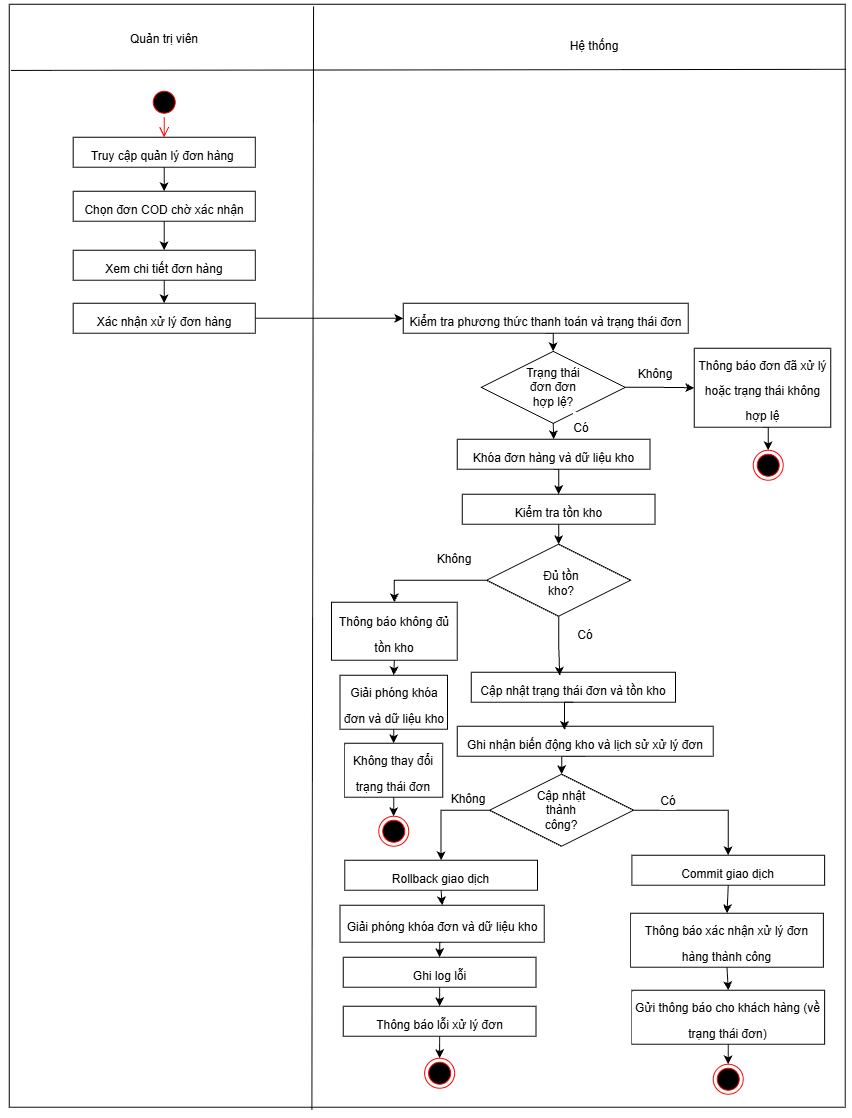
\includegraphics[width=0.94\textwidth,height=0.58\textheight,keepaspectratio]{Images/Activity/da-Xử lý và xác nhận đơn COD.drawio.png}
    \captionof{figure}{Sơ đồ hoạt động xử lý và xác nhận đơn COD}
    \label{appendix:fig:activity-cod-confirmation}
\end{minipage}
\par\medskip

\par\medskip\noindent
\begin{minipage}{\textwidth}
\subsubsection{Đồng bộ chỉ mục AI}

Quản trị viên khởi tạo tác vụ đồng bộ; Backend lấy dữ liệu sản phẩm từ MySQL và
AI Service cập nhật vector trong Qdrant theo từng lô. Sản phẩm lỗi được ghi nhận
để thử lại mà không làm dừng toàn bộ tác vụ.

\centering
    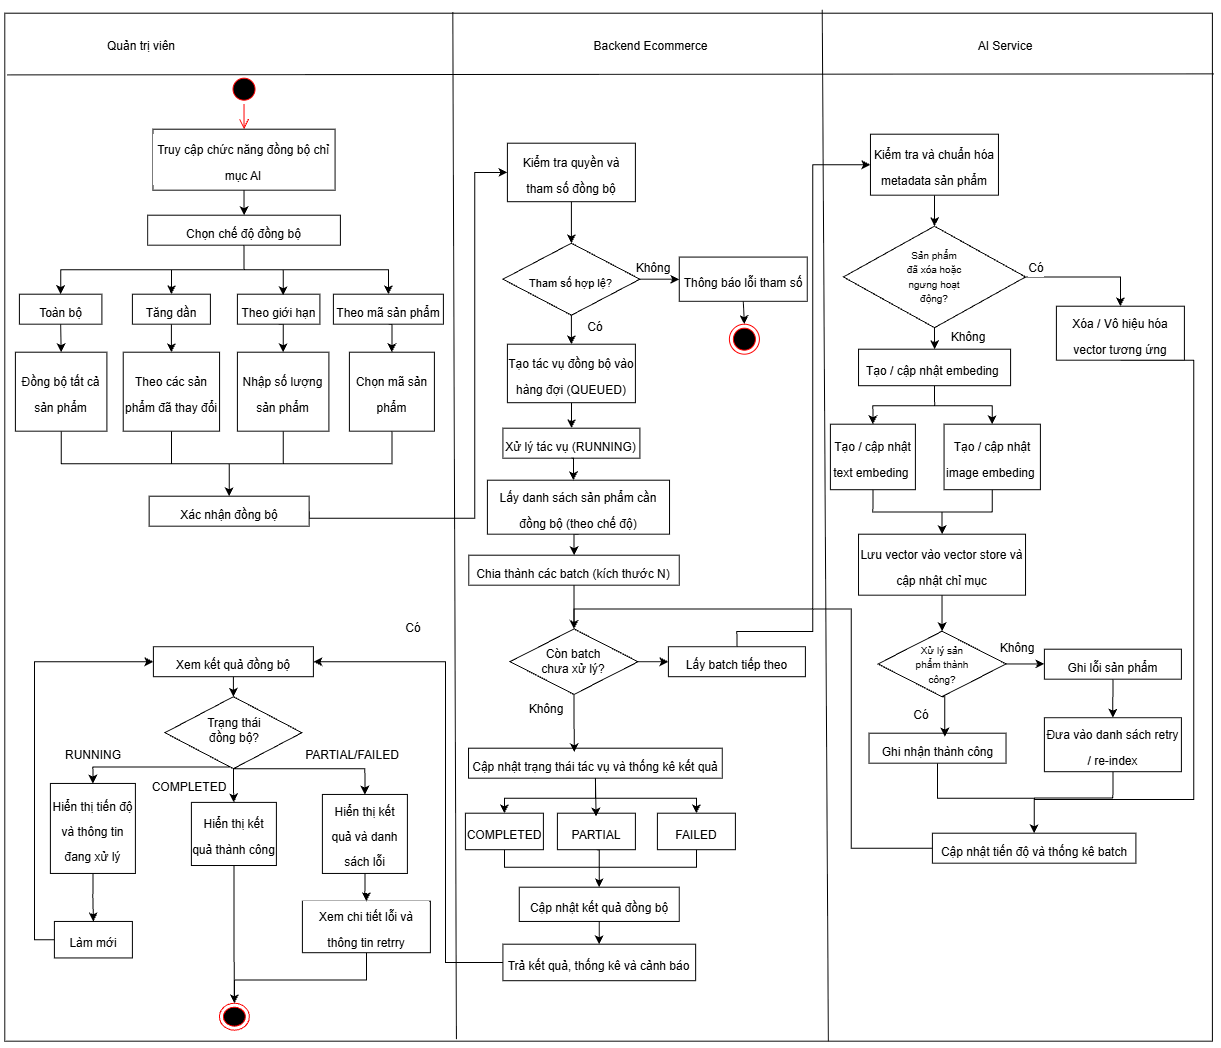
\includegraphics[width=0.94\textwidth,height=0.58\textheight,keepaspectratio]{Images/Activity/da-Đồng bộ chỉ mục AI.drawio.png}
    \captionof{figure}{Sơ đồ hoạt động đồng bộ chỉ mục AI}
    \label{appendix:fig:activity-ai-index-sync}
\end{minipage}
\par\medskip

\FloatBarrier

%=========================
% Appendices/03-ThietKeDuLieu.tex
% Phụ lục C -- Thiết kế dữ liệu và từ điển dữ liệu
%=========================

\section{Thiết kế dữ liệu và từ điển dữ liệu}
\label{data-dictionary}

Phụ lục này trình bày từ điển dữ liệu chi tiết của hệ thống theo từng miền
nghiệp vụ. Mỗi bảng được mô tả bằng tên trường, kiểu dữ liệu và ý nghĩa sử dụng;
các bảng có quan hệ với nhau được giữ trong cùng nhóm để thuận tiện đối chiếu
với sơ đồ dữ liệu tổng quan ở Chương 5.

\subsection{Người dùng và phân quyền}
% Tệp được tách theo nhóm để duy trì từ điển dữ liệu của Chương 5.

\begin{longtable}{|>{\RaggedRight\arraybackslash}p{0.25\textwidth}|>{\RaggedRight\arraybackslash}p{0.20\textwidth}|>{\RaggedRight\arraybackslash}p{0.45\textwidth}|}
    \caption{Mô tả chi tiết bảng \texttt{user\_accounts} (Tài khoản người dùng)}
    \label{tab:data-dictionary-user-accounts} \\
    \hline
    \textbf{Tên trường} & \textbf{Kiểu dữ liệu} & \textbf{Mô tả} \\
    \hline
    \endfirsthead
    \multicolumn{3}{c}{\tablename\ \thetable\ (tiếp theo)} \\
    \hline
    \textbf{Tên trường} & \textbf{Kiểu dữ liệu} & \textbf{Mô tả} \\
    \hline
    \endhead
    \texttt{\seqsplit{id}} & \texttt{bigint} & Khóa chính tự tăng. \\
        \hline
        \texttt{\seqsplit{email}} & \texttt{varchar(320)} & Địa chỉ thư điện tử; bắt buộc; duy nhất. \\
        \hline
        \texttt{\seqsplit{phone\_number}} & \texttt{varchar(30)} & Số điện thoại; duy nhất. \\
        \hline
        \texttt{\seqsplit{password\_hash}} & \texttt{varchar(255)} & Giá trị băm của mật khẩu; bắt buộc. \\
        \hline
        \texttt{\seqsplit{password\_login\_enabled}} & \texttt{boolean} & Cho biết tài khoản có cho phép đăng nhập bằng mật khẩu. \\
        \hline
        \texttt{\seqsplit{full\_name}} & \texttt{varchar(150)} & Họ và tên đầy đủ. \\
        \hline
        \texttt{\seqsplit{display\_name}} & \texttt{varchar(150)} & Tên hiển thị. \\
        \hline
        \texttt{\seqsplit{status}} & \texttt{varchar(50)} & Trạng thái hiện tại; bắt buộc. \\
        \hline
        \texttt{\seqsplit{email\_verified}} & \texttt{boolean} & Cho biết email đã được xác minh. \\
        \hline
        \texttt{\seqsplit{phone\_verified}} & \texttt{boolean} & Cho biết số điện thoại đã được xác minh. \\
        \hline
        \texttt{\seqsplit{last\_login\_at}} & \texttt{datetime(6)} & Thời điểm đăng nhập gần nhất. \\
        \hline
        \texttt{\seqsplit{created\_at}} & \texttt{datetime(6)} & Thời điểm tạo bản ghi. \\
        \hline
        \texttt{\seqsplit{updated\_at}} & \texttt{datetime(6)} & Thời điểm cập nhật gần nhất. \\
        \hline
\end{longtable}

\begin{longtable}{|>{\RaggedRight\arraybackslash}p{0.25\textwidth}|>{\RaggedRight\arraybackslash}p{0.20\textwidth}|>{\RaggedRight\arraybackslash}p{0.45\textwidth}|}
    \caption{Mô tả chi tiết bảng \texttt{user\_roles} (Vai trò người dùng)}
    \label{tab:data-dictionary-user-roles} \\
    \hline
    \textbf{Tên trường} & \textbf{Kiểu dữ liệu} & \textbf{Mô tả} \\
    \hline
    \endfirsthead
    \multicolumn{3}{c}{\tablename\ \thetable\ (tiếp theo)} \\
    \hline
    \textbf{Tên trường} & \textbf{Kiểu dữ liệu} & \textbf{Mô tả} \\
    \hline
    \endhead
    \texttt{\seqsplit{id}} & \texttt{bigint} & Khóa chính tự tăng. \\
        \hline
        \texttt{\seqsplit{name}} & \texttt{varchar(100)} & Tên; bắt buộc; duy nhất. \\
        \hline
        \texttt{\seqsplit{description}} & \texttt{varchar(255)} & Nội dung mô tả. \\
        \hline
        \texttt{\seqsplit{active}} & \texttt{boolean} & Cho biết bản ghi đang hoạt động. \\
        \hline
        \texttt{\seqsplit{created\_at}} & \texttt{datetime(6)} & Thời điểm tạo bản ghi. \\
        \hline
        \texttt{\seqsplit{updated\_at}} & \texttt{datetime(6)} & Thời điểm cập nhật gần nhất. \\
        \hline
\end{longtable}

\begin{longtable}{|>{\RaggedRight\arraybackslash}p{0.25\textwidth}|>{\RaggedRight\arraybackslash}p{0.20\textwidth}|>{\RaggedRight\arraybackslash}p{0.45\textwidth}|}
    \caption{Mô tả chi tiết bảng \texttt{user\_account\_roles} (Gán vai trò cho tài khoản)}
    \label{tab:data-dictionary-user-account-roles} \\
    \hline
    \textbf{Tên trường} & \textbf{Kiểu dữ liệu} & \textbf{Mô tả} \\
    \hline
    \endfirsthead
    \multicolumn{3}{c}{\tablename\ \thetable\ (tiếp theo)} \\
    \hline
    \textbf{Tên trường} & \textbf{Kiểu dữ liệu} & \textbf{Mô tả} \\
    \hline
    \endhead
    \texttt{\seqsplit{user\_account\_id}} & \texttt{bigint} & Khóa ngoại tham chiếu \texttt{user\_accounts.id}; bắt buộc. \\
        \hline
        \texttt{\seqsplit{role\_id}} & \texttt{bigint} & Khóa ngoại tham chiếu \texttt{user\_roles.id}; bắt buộc. \\
        \hline
\end{longtable}

\begin{longtable}{|>{\RaggedRight\arraybackslash}p{0.25\textwidth}|>{\RaggedRight\arraybackslash}p{0.20\textwidth}|>{\RaggedRight\arraybackslash}p{0.45\textwidth}|}
    \caption{Mô tả chi tiết bảng \texttt{customer\_profiles} (Hồ sơ khách hàng)}
    \label{tab:data-dictionary-customer-profiles} \\
    \hline
    \textbf{Tên trường} & \textbf{Kiểu dữ liệu} & \textbf{Mô tả} \\
    \hline
    \endfirsthead
    \multicolumn{3}{c}{\tablename\ \thetable\ (tiếp theo)} \\
    \hline
    \textbf{Tên trường} & \textbf{Kiểu dữ liệu} & \textbf{Mô tả} \\
    \hline
    \endhead
    \texttt{\seqsplit{id}} & \texttt{bigint} & Khóa chính tự tăng. \\
        \hline
        \texttt{\seqsplit{user\_account\_id}} & \texttt{bigint} & Khóa ngoại tham chiếu \texttt{user\_accounts.id}; bắt buộc; duy nhất. \\
        \hline
        \texttt{\seqsplit{first\_name}} & \texttt{varchar(100)} & Tên. \\
        \hline
        \texttt{\seqsplit{last\_name}} & \texttt{varchar(100)} & Họ. \\
        \hline
        \texttt{\seqsplit{gender}} & \texttt{varchar(50)} & Giới tính. \\
        \hline
        \texttt{\seqsplit{date\_of\_birth}} & \texttt{date} & Ngày sinh. \\
        \hline
        \texttt{\seqsplit{avatar\_url}} & \texttt{text} & Đường dẫn ảnh đại diện. \\
        \hline
        \texttt{\seqsplit{loyalty\_points}} & \texttt{int} & Điểm khách hàng thân thiết. \\
        \hline
        \texttt{\seqsplit{marketing\_opt\_in}} & \texttt{boolean} & Cho biết khách hàng đồng ý nhận nội dung tiếp thị. \\
        \hline
        \texttt{\seqsplit{created\_at}} & \texttt{datetime(6)} & Thời điểm tạo bản ghi. \\
        \hline
        \texttt{\seqsplit{updated\_at}} & \texttt{datetime(6)} & Thời điểm cập nhật gần nhất. \\
        \hline
\end{longtable}

\begin{longtable}{|>{\RaggedRight\arraybackslash}p{0.25\textwidth}|>{\RaggedRight\arraybackslash}p{0.20\textwidth}|>{\RaggedRight\arraybackslash}p{0.45\textwidth}|}
    \caption{Mô tả chi tiết bảng \texttt{customer\_addresses} (Địa chỉ khách hàng)}
    \label{tab:data-dictionary-customer-addresses} \\
    \hline
    \textbf{Tên trường} & \textbf{Kiểu dữ liệu} & \textbf{Mô tả} \\
    \hline
    \endfirsthead
    \multicolumn{3}{c}{\tablename\ \thetable\ (tiếp theo)} \\
    \hline
    \textbf{Tên trường} & \textbf{Kiểu dữ liệu} & \textbf{Mô tả} \\
    \hline
    \endhead
    \texttt{\seqsplit{id}} & \texttt{bigint} & Khóa chính tự tăng. \\
        \hline
        \texttt{\seqsplit{user\_account\_id}} & \texttt{bigint} & Khóa ngoại tham chiếu \texttt{user\_accounts.id}; bắt buộc. \\
        \hline
        \texttt{\seqsplit{address\_type}} & \texttt{varchar(50)} & Loại địa chỉ; bắt buộc. \\
        \hline
        \texttt{\seqsplit{recipient\_name}} & \texttt{varchar(150)} & Tên người nhận; bắt buộc. \\
        \hline
        \texttt{\seqsplit{phone\_number}} & \texttt{varchar(30)} & Số điện thoại; bắt buộc. \\
        \hline
        \texttt{\seqsplit{address\_line1}} & \texttt{varchar(255)} & Dòng địa chỉ chính; bắt buộc. \\
        \hline
        \texttt{\seqsplit{address\_line2}} & \texttt{varchar(255)} & Dòng địa chỉ bổ sung. \\
        \hline
        \texttt{\seqsplit{ward}} & \texttt{varchar(150)} & Phường hoặc xã. \\
        \hline
        \texttt{\seqsplit{district}} & \texttt{varchar(150)} & Quận hoặc huyện. \\
        \hline
        \texttt{\seqsplit{city}} & \texttt{varchar(150)} & Thành phố. \\
        \hline
        \texttt{\seqsplit{province}} & \texttt{varchar(150)} & Tỉnh hoặc thành phố trực thuộc trung ương. \\
        \hline
        \texttt{\seqsplit{country\_code}} & \texttt{varchar(2)} & Mã quốc gia hai ký tự; bắt buộc. \\
        \hline
        \texttt{\seqsplit{postal\_code}} & \texttt{varchar(20)} & Mã bưu chính. \\
        \hline
        \texttt{\seqsplit{is\_default}} & \texttt{boolean} & Cho biết đây là bản ghi mặc định. \\
        \hline
        \texttt{\seqsplit{deleted}} & \texttt{boolean} & Đánh dấu xóa mềm. \\
        \hline
        \texttt{\seqsplit{created\_at}} & \texttt{datetime(6)} & Thời điểm tạo bản ghi. \\
        \hline
        \texttt{\seqsplit{updated\_at}} & \texttt{datetime(6)} & Thời điểm cập nhật gần nhất. \\
        \hline
\end{longtable}

\begin{longtable}{|>{\RaggedRight\arraybackslash}p{0.25\textwidth}|>{\RaggedRight\arraybackslash}p{0.20\textwidth}|>{\RaggedRight\arraybackslash}p{0.45\textwidth}|}
    \caption{Mô tả chi tiết bảng \texttt{refresh\_tokens} (Refresh token)}
    \label{tab:data-dictionary-refresh-tokens} \\
    \hline
    \textbf{Tên trường} & \textbf{Kiểu dữ liệu} & \textbf{Mô tả} \\
    \hline
    \endfirsthead
    \multicolumn{3}{c}{\tablename\ \thetable\ (tiếp theo)} \\
    \hline
    \textbf{Tên trường} & \textbf{Kiểu dữ liệu} & \textbf{Mô tả} \\
    \hline
    \endhead
    \texttt{\seqsplit{id}} & \texttt{bigint} & Khóa chính tự tăng. \\
        \hline
        \texttt{\seqsplit{user\_account\_id}} & \texttt{bigint} & Khóa ngoại tham chiếu \texttt{user\_accounts.id}; bắt buộc. \\
        \hline
        \texttt{\seqsplit{token\_hash}} & \texttt{varchar(255)} & Giá trị băm của token; bắt buộc; duy nhất. \\
        \hline
        \texttt{\seqsplit{status}} & \texttt{varchar(50)} & Trạng thái hiện tại; bắt buộc. \\
        \hline
        \texttt{\seqsplit{issued\_at}} & \texttt{datetime(6)} & Thời điểm phát hành. \\
        \hline
        \texttt{\seqsplit{expires\_at}} & \texttt{datetime(6)} & Thời điểm hết hiệu lực; bắt buộc. \\
        \hline
        \texttt{\seqsplit{revoked\_at}} & \texttt{datetime(6)} & Thời điểm bị thu hồi. \\
        \hline
        \texttt{\seqsplit{replaced\_by\_token\_hash}} & \texttt{varchar(255)} & Giá trị băm của token thay thế. \\
        \hline
        \texttt{\seqsplit{ip\_address}} & \texttt{varchar(45)} & Địa chỉ IP tạo token. \\
        \hline
        \texttt{\seqsplit{user\_agent}} & \texttt{text} & Thông tin thiết bị và trình duyệt. \\
        \hline
        \texttt{\seqsplit{created\_at}} & \texttt{datetime(6)} & Thời điểm tạo bản ghi. \\
        \hline
        \texttt{\seqsplit{updated\_at}} & \texttt{datetime(6)} & Thời điểm cập nhật gần nhất. \\
        \hline
\end{longtable}

\begin{longtable}{|>{\RaggedRight\arraybackslash}p{0.25\textwidth}|>{\RaggedRight\arraybackslash}p{0.20\textwidth}|>{\RaggedRight\arraybackslash}p{0.45\textwidth}|}
    \caption{Mô tả chi tiết bảng \texttt{password\_reset\_otps} (Mã OTP đặt lại mật khẩu)}
    \label{tab:data-dictionary-password-reset-otps} \\
    \hline
    \textbf{Tên trường} & \textbf{Kiểu dữ liệu} & \textbf{Mô tả} \\
    \hline
    \endfirsthead
    \multicolumn{3}{c}{\tablename\ \thetable\ (tiếp theo)} \\
    \hline
    \textbf{Tên trường} & \textbf{Kiểu dữ liệu} & \textbf{Mô tả} \\
    \hline
    \endhead
    \texttt{\seqsplit{id}} & \texttt{bigint} & Khóa chính tự tăng. \\
        \hline
        \texttt{\seqsplit{user\_account\_id}} & \texttt{bigint} & Khóa ngoại tham chiếu \texttt{user\_accounts.id}; bắt buộc. \\
        \hline
        \texttt{\seqsplit{email}} & \texttt{varchar(320)} & Địa chỉ thư điện tử; bắt buộc. \\
        \hline
        \texttt{\seqsplit{otp\_hash}} & \texttt{varchar(255)} & Giá trị băm của mã OTP; bắt buộc. \\
        \hline
        \texttt{\seqsplit{reset\_token\_hash}} & \texttt{varchar(255)} & Giá trị băm của token đặt lại mật khẩu. \\
        \hline
        \texttt{\seqsplit{failed\_attempts}} & \texttt{int} & Số lần xác thực thất bại; bắt buộc. \\
        \hline
        \texttt{\seqsplit{max\_failed\_attempts}} & \texttt{int} & Số lần xác thực thất bại tối đa; bắt buộc. \\
        \hline
        \texttt{\seqsplit{expires\_at}} & \texttt{datetime(6)} & Thời điểm hết hiệu lực; bắt buộc. \\
        \hline
        \texttt{\seqsplit{reset\_token\_expires\_at}} & \texttt{datetime(6)} & Thời điểm token đặt lại mật khẩu hết hạn. \\
        \hline
        \texttt{\seqsplit{verified\_at}} & \texttt{datetime(6)} & Thời điểm xác minh thành công. \\
        \hline
        \texttt{\seqsplit{used\_at}} & \texttt{datetime(6)} & Thời điểm đã sử dụng. \\
        \hline
        \texttt{\seqsplit{created\_at}} & \texttt{datetime(6)} & Thời điểm tạo bản ghi. \\
        \hline
        \texttt{\seqsplit{updated\_at}} & \texttt{datetime(6)} & Thời điểm cập nhật gần nhất. \\
        \hline
\end{longtable}


\subsection{Danh mục và sản phẩm}
% Tệp được tách theo nhóm để duy trì từ điển dữ liệu của Chương 5.

\begin{longtable}{|>{\RaggedRight\arraybackslash}p{0.25\textwidth}|>{\RaggedRight\arraybackslash}p{0.20\textwidth}|>{\RaggedRight\arraybackslash}p{0.45\textwidth}|}
    \caption{Mô tả chi tiết bảng \texttt{products} (Sản phẩm)}
    \label{tab:data-dictionary-products} \\
    \hline
    \textbf{Tên trường} & \textbf{Kiểu dữ liệu} & \textbf{Mô tả} \\
    \hline
    \endfirsthead
    \multicolumn{3}{c}{\tablename\ \thetable\ (tiếp theo)} \\
    \hline
    \textbf{Tên trường} & \textbf{Kiểu dữ liệu} & \textbf{Mô tả} \\
    \hline
    \endhead
    \texttt{\seqsplit{id}} & \texttt{bigint} & Khóa chính. \\
        \hline
        \texttt{\seqsplit{age\_group}} & \texttt{varchar(100)} & Nhóm tuổi của sản phẩm. \\
        \hline
        \texttt{\seqsplit{age\_group\_vi}} & \texttt{varchar(100)} & Nhóm tuổi bằng tiếng Việt. \\
        \hline
        \texttt{\seqsplit{article\_number}} & \texttt{varchar(100)} & Mã bài hàng của sản phẩm. \\
        \hline
        \texttt{\seqsplit{base\_colour}} & \texttt{varchar(100)} & Màu cơ bản. \\
        \hline
        \texttt{\seqsplit{base\_colour\_vi}} & \texttt{varchar(100)} & Màu cơ bản bằng tiếng Việt. \\
        \hline
        \texttt{\seqsplit{brand\_name}} & \texttt{varchar(150)} & Tên thương hiệu. \\
        \hline
        \texttt{\seqsplit{catalog\_add\_date}} & \texttt{datetime(6)} & Thời điểm sản phẩm được thêm vào danh mục. \\
        \hline
        \texttt{\seqsplit{colour1}} & \texttt{varchar(100)} & Màu thứ nhất. \\
        \hline
        \texttt{\seqsplit{colour1\_vi}} & \texttt{varchar(100)} & Màu thứ nhất bằng tiếng Việt. \\
        \hline
        \texttt{\seqsplit{colour2}} & \texttt{varchar(100)} & Màu thứ hai. \\
        \hline
        \texttt{\seqsplit{colour2\_vi}} & \texttt{varchar(100)} & Màu thứ hai bằng tiếng Việt. \\
        \hline
        \texttt{\seqsplit{created\_at}} & \texttt{datetime(6)} & Thời điểm tạo bản ghi. \\
        \hline
        \texttt{\seqsplit{description}} & \texttt{text} & Nội dung mô tả. \\
        \hline
        \texttt{\seqsplit{description\_vi}} & \texttt{text} & Mô tả bằng tiếng Việt. \\
        \hline
        \texttt{\seqsplit{external\_id}} & \texttt{bigint} & Định danh sản phẩm tại nguồn ngoài. \\
        \hline
        \texttt{\seqsplit{fit}} & \texttt{varchar(150)} & Kiểu dáng. \\
        \hline
        \texttt{\seqsplit{fit\_vi}} & \texttt{varchar(150)} & Kiểu dáng bằng tiếng Việt. \\
        \hline
        \texttt{\seqsplit{gender}} & \texttt{varchar(50)} & Giới tính. \\
        \hline
        \texttt{\seqsplit{gender\_vi}} & \texttt{varchar(50)} & Giới tính bằng tiếng Việt. \\
        \hline
        \texttt{\seqsplit{main\_image}} & \texttt{text} & Đường dẫn ảnh đại diện chính. \\
        \hline
        \texttt{\seqsplit{material}} & \texttt{varchar(150)} & Chất liệu. \\
        \hline
        \texttt{\seqsplit{material\_vi}} & \texttt{varchar(150)} & Chất liệu bằng tiếng Việt. \\
        \hline
        \texttt{\seqsplit{product\_display\_name}} & \texttt{varchar(255)} & Tên hiển thị của sản phẩm; bắt buộc. \\
        \hline
        \texttt{\seqsplit{product\_display\_name\_vi}} & \texttt{varchar(255)} & Tên hiển thị bằng tiếng Việt. \\
        \hline
        \texttt{\seqsplit{product\_usage}} & \texttt{varchar(100)} & Mục đích sử dụng. \\
        \hline
        \texttt{\seqsplit{product\_usage\_vi}} & \texttt{varchar(100)} & Mục đích sử dụng bằng tiếng Việt. \\
        \hline
        \texttt{\seqsplit{season}} & \texttt{varchar(50)} & Mùa sử dụng. \\
        \hline
        \texttt{\seqsplit{season\_vi}} & \texttt{varchar(50)} & Mùa sử dụng bằng tiếng Việt. \\
        \hline
        \texttt{\seqsplit{updated\_at}} & \texttt{datetime(6)} & Thời điểm cập nhật gần nhất. \\
        \hline
        \texttt{\seqsplit{variant\_name}} & \texttt{varchar(255)} & Tên biến thể. \\
        \hline
        \texttt{\seqsplit{variant\_name\_vi}} & \texttt{varchar(255)} & Tên biến thể bằng tiếng Việt. \\
        \hline
        \texttt{\seqsplit{year}} & \texttt{int} & Năm của mẫu sản phẩm. \\
        \hline
\end{longtable}

\begin{longtable}{|>{\RaggedRight\arraybackslash}p{0.25\textwidth}|>{\RaggedRight\arraybackslash}p{0.20\textwidth}|>{\RaggedRight\arraybackslash}p{0.45\textwidth}|}
    \caption{Mô tả chi tiết bảng \texttt{categories} (Danh mục sản phẩm)}
    \label{tab:data-dictionary-categories} \\
    \hline
    \textbf{Tên trường} & \textbf{Kiểu dữ liệu} & \textbf{Mô tả} \\
    \hline
    \endfirsthead
    \multicolumn{3}{c}{\tablename\ \thetable\ (tiếp theo)} \\
    \hline
    \textbf{Tên trường} & \textbf{Kiểu dữ liệu} & \textbf{Mô tả} \\
    \hline
    \endhead
    \texttt{\seqsplit{id}} & \texttt{bigint} & Khóa chính tự tăng. \\
        \hline
        \texttt{\seqsplit{source\_category\_id}} & \texttt{bigint} & Định danh danh mục tại nguồn dữ liệu ngoài. \\
        \hline
        \texttt{\seqsplit{category\_level}} & \texttt{varchar(50)} & Cấp của danh mục; bắt buộc. \\
        \hline
        \texttt{\seqsplit{category\_name}} & \texttt{varchar(150)} & Tên danh mục; bắt buộc. \\
        \hline
        \texttt{\seqsplit{is\_active}} & \texttt{boolean} & Cho biết danh mục đang được kích hoạt và có thể sử dụng. \\
        \hline
        \texttt{\seqsplit{category\_name\_vi}} & \texttt{varchar(150)} & Tên danh mục bằng tiếng Việt. \\
        \hline
        \texttt{\seqsplit{parent\_id}} & \texttt{bigint} & Khóa ngoại tham chiếu \texttt{categories.id}. \\
        \hline
        \texttt{\seqsplit{canonical\_code}} & \texttt{varchar(100)} & Mã chuẩn duy nhất của danh mục; duy nhất. \\
        \hline
\end{longtable}

\begin{longtable}{|>{\RaggedRight\arraybackslash}p{0.25\textwidth}|>{\RaggedRight\arraybackslash}p{0.20\textwidth}|>{\RaggedRight\arraybackslash}p{0.45\textwidth}|}
    \caption{Mô tả chi tiết bảng \texttt{product\_categories} (Liên kết sản phẩm--danh mục)}
    \label{tab:data-dictionary-product-categories} \\
    \hline
    \textbf{Tên trường} & \textbf{Kiểu dữ liệu} & \textbf{Mô tả} \\
    \hline
    \endfirsthead
    \multicolumn{3}{c}{\tablename\ \thetable\ (tiếp theo)} \\
    \hline
    \textbf{Tên trường} & \textbf{Kiểu dữ liệu} & \textbf{Mô tả} \\
    \hline
    \endhead
    \texttt{\seqsplit{id}} & \texttt{bigint} & Khóa chính tự tăng. \\
        \hline
        \texttt{\seqsplit{product\_id}} & \texttt{bigint} & Khóa ngoại tham chiếu \texttt{products.id}; bắt buộc. \\
        \hline
        \texttt{\seqsplit{category\_id}} & \texttt{bigint} & Khóa ngoại tham chiếu \texttt{categories.id}; bắt buộc. \\
        \hline
\end{longtable}

\begin{longtable}{|>{\RaggedRight\arraybackslash}p{0.25\textwidth}|>{\RaggedRight\arraybackslash}p{0.20\textwidth}|>{\RaggedRight\arraybackslash}p{0.45\textwidth}|}
    \caption{Mô tả chi tiết bảng \texttt{product\_variants} (Biến thể sản phẩm)}
    \label{tab:data-dictionary-product-variants} \\
    \hline
    \textbf{Tên trường} & \textbf{Kiểu dữ liệu} & \textbf{Mô tả} \\
    \hline
    \endfirsthead
    \multicolumn{3}{c}{\tablename\ \thetable\ (tiếp theo)} \\
    \hline
    \textbf{Tên trường} & \textbf{Kiểu dữ liệu} & \textbf{Mô tả} \\
    \hline
    \endhead
    \texttt{\seqsplit{id}} & \texttt{bigint} & Khóa chính tự tăng. \\
        \hline
        \texttt{\seqsplit{product\_id}} & \texttt{bigint} & Khóa ngoại tham chiếu \texttt{products.id}; bắt buộc. \\
        \hline
        \texttt{\seqsplit{sku\_id}} & \texttt{bigint} & Định danh SKU; duy nhất. \\
        \hline
        \texttt{\seqsplit{option\_name}} & \texttt{varchar(100)} & Tên tùy chọn biến thể. \\
        \hline
        \texttt{\seqsplit{option\_value}} & \texttt{varchar(100)} & Giá trị tùy chọn biến thể. \\
        \hline
        \texttt{\seqsplit{unified\_size}} & \texttt{varchar(100)} & Kích cỡ đã chuẩn hóa. \\
        \hline
        \texttt{\seqsplit{inventory\_count}} & \texttt{int} & Số lượng tồn hiện hành. \\
        \hline
        \texttt{\seqsplit{available}} & \texttt{boolean} & Cho biết biến thể còn khả dụng. \\
        \hline
        \texttt{\seqsplit{active}} & \texttt{boolean} & Cho biết bản ghi đang hoạt động. \\
        \hline
        \texttt{\seqsplit{created\_at}} & \texttt{timestamp} & Thời điểm tạo bản ghi. \\
        \hline
        \texttt{\seqsplit{updated\_at}} & \texttt{timestamp} & Thời điểm cập nhật gần nhất. \\
        \hline
\end{longtable}

\begin{longtable}{|>{\RaggedRight\arraybackslash}p{0.25\textwidth}|>{\RaggedRight\arraybackslash}p{0.20\textwidth}|>{\RaggedRight\arraybackslash}p{0.45\textwidth}|}
    \caption{Mô tả chi tiết bảng \texttt{product\_attributes} (Thuộc tính sản phẩm)}
    \label{tab:data-dictionary-product-attributes} \\
    \hline
    \textbf{Tên trường} & \textbf{Kiểu dữ liệu} & \textbf{Mô tả} \\
    \hline
    \endfirsthead
    \multicolumn{3}{c}{\tablename\ \thetable\ (tiếp theo)} \\
    \hline
    \textbf{Tên trường} & \textbf{Kiểu dữ liệu} & \textbf{Mô tả} \\
    \hline
    \endhead
    \texttt{\seqsplit{id}} & \texttt{bigint} & Khóa chính tự tăng. \\
        \hline
        \texttt{\seqsplit{product\_id}} & \texttt{bigint} & Khóa ngoại tham chiếu \texttt{products.id}; bắt buộc. \\
        \hline
        \texttt{\seqsplit{attr\_key}} & \texttt{varchar(255)} & Tên thuộc tính; bắt buộc. \\
        \hline
        \texttt{\seqsplit{attr\_value}} & \texttt{text} & Giá trị thuộc tính. \\
        \hline
        \texttt{\seqsplit{created\_at}} & \texttt{timestamp} & Thời điểm tạo bản ghi. \\
        \hline
        \texttt{\seqsplit{updated\_at}} & \texttt{timestamp} & Thời điểm cập nhật gần nhất. \\
        \hline
        \texttt{\seqsplit{attr\_value\_vi}} & \texttt{text} & Giá trị thuộc tính bằng tiếng Việt. \\
        \hline
\end{longtable}

\begin{longtable}{|>{\RaggedRight\arraybackslash}p{0.25\textwidth}|>{\RaggedRight\arraybackslash}p{0.20\textwidth}|>{\RaggedRight\arraybackslash}p{0.45\textwidth}|}
    \caption{Mô tả chi tiết bảng \texttt{product\_images} (Hình ảnh sản phẩm)}
    \label{tab:data-dictionary-product-images} \\
    \hline
    \textbf{Tên trường} & \textbf{Kiểu dữ liệu} & \textbf{Mô tả} \\
    \hline
    \endfirsthead
    \multicolumn{3}{c}{\tablename\ \thetable\ (tiếp theo)} \\
    \hline
    \textbf{Tên trường} & \textbf{Kiểu dữ liệu} & \textbf{Mô tả} \\
    \hline
    \endhead
    \texttt{\seqsplit{id}} & \texttt{bigint} & Khóa chính tự tăng. \\
        \hline
        \texttt{\seqsplit{product\_id}} & \texttt{bigint} & Khóa ngoại tham chiếu \texttt{products.id}; bắt buộc. \\
        \hline
        \texttt{\seqsplit{image\_type}} & \texttt{varchar(50)} & Loại hình ảnh; bắt buộc. \\
        \hline
        \texttt{\seqsplit{image\_url}} & \texttt{text} & Đường dẫn hình ảnh; bắt buộc. \\
        \hline
        \texttt{\seqsplit{sort\_order}} & \texttt{int} & Thứ tự hiển thị. \\
        \hline
        \texttt{\seqsplit{created\_at}} & \texttt{timestamp} & Thời điểm tạo bản ghi. \\
        \hline
\end{longtable}

\begin{longtable}{|>{\RaggedRight\arraybackslash}p{0.25\textwidth}|>{\RaggedRight\arraybackslash}p{0.20\textwidth}|>{\RaggedRight\arraybackslash}p{0.45\textwidth}|}
    \caption{Mô tả chi tiết bảng \texttt{product\_prices} (Giá sản phẩm)}
    \label{tab:data-dictionary-product-prices} \\
    \hline
    \textbf{Tên trường} & \textbf{Kiểu dữ liệu} & \textbf{Mô tả} \\
    \hline
    \endfirsthead
    \multicolumn{3}{c}{\tablename\ \thetable\ (tiếp theo)} \\
    \hline
    \textbf{Tên trường} & \textbf{Kiểu dữ liệu} & \textbf{Mô tả} \\
    \hline
    \endhead
    \texttt{\seqsplit{id}} & \texttt{bigint} & Khóa chính tự tăng. \\
        \hline
        \texttt{\seqsplit{product\_id}} & \texttt{bigint} & Khóa ngoại tham chiếu \texttt{products.id}; bắt buộc. \\
        \hline
        \texttt{\seqsplit{selling\_price}} & \texttt{decimal(12,2)} & Giá bán; bắt buộc. \\
        \hline
        \texttt{\seqsplit{import\_price}} & \texttt{decimal(12,2)} & Giá nhập. \\
        \hline
        \texttt{\seqsplit{vat}} & \texttt{decimal(8,2)} & Thuế giá trị gia tăng. \\
        \hline
        \texttt{\seqsplit{created\_at}} & \texttt{timestamp} & Thời điểm tạo bản ghi. \\
        \hline
        \texttt{\seqsplit{updated\_at}} & \texttt{timestamp} & Thời điểm cập nhật gần nhất. \\
        \hline
\end{longtable}


\subsection{Quản lý kho}
% Tệp được tách theo nhóm để duy trì từ điển dữ liệu của Chương 6.

\begin{longtable}{|>{\RaggedRight\arraybackslash}p{0.25\textwidth}|>{\RaggedRight\arraybackslash}p{0.20\textwidth}|>{\RaggedRight\arraybackslash}p{0.45\textwidth}|}
    \caption{Mô tả chi tiết bảng \texttt{inventory\_reservations} (Giữ tồn kho)}
    \label{tab:data-dictionary-inventory-reservations} \\
    \hline
    \textbf{Tên trường} & \textbf{Kiểu dữ liệu} & \textbf{Mô tả} \\
    \hline
    \endfirsthead
    \multicolumn{3}{c}{\tablename\ \thetable\ (tiếp theo)} \\
    \hline
    \textbf{Tên trường} & \textbf{Kiểu dữ liệu} & \textbf{Mô tả} \\
    \hline
    \endhead
    \texttt{\seqsplit{id}} & \texttt{bigint} & Khóa chính tự tăng. \\
        \hline
        \texttt{\seqsplit{product\_id}} & \texttt{bigint} & Khóa ngoại tham chiếu \texttt{products.id}; bắt buộc. \\
        \hline
        \texttt{\seqsplit{product\_variant\_id}} & \texttt{bigint} & Khóa ngoại tham chiếu \texttt{product\_variants.id}; bắt buộc. \\
        \hline
        \texttt{\seqsplit{user\_account\_id}} & \texttt{bigint} & Khóa ngoại tham chiếu \texttt{user\_accounts.id}; bắt buộc. \\
        \hline
        \texttt{\seqsplit{cart\_id}} & \texttt{bigint} & Khóa ngoại tham chiếu \texttt{carts.id}. \\
        \hline
        \texttt{\seqsplit{order\_id}} & \texttt{bigint} & Khóa ngoại tham chiếu \texttt{orders.id}. \\
        \hline
        \texttt{\seqsplit{reservation\_key}} & \texttt{varchar(100)} & Khóa duy nhất chống giữ tồn kho trùng; duy nhất. \\
        \hline
        \texttt{\seqsplit{quantity}} & \texttt{int} & Số lượng; bắt buộc. \\
        \hline
        \texttt{\seqsplit{status}} & \texttt{varchar(50)} & Trạng thái hiện tại; bắt buộc. \\
        \hline
        \texttt{\seqsplit{reserved\_at}} & \texttt{datetime(6)} & Thời điểm giữ hàng. \\
        \hline
        \texttt{\seqsplit{expires\_at}} & \texttt{datetime(6)} & Thời điểm hết hiệu lực. \\
        \hline
        \texttt{\seqsplit{consumed\_at}} & \texttt{datetime(6)} & Thời điểm phần giữ hàng được sử dụng. \\
        \hline
        \texttt{\seqsplit{released\_at}} & \texttt{datetime(6)} & Thời điểm giải phóng phần giữ hàng. \\
        \hline
        \texttt{\seqsplit{release\_reason}} & \texttt{varchar(150)} & Lý do giải phóng. \\
        \hline
        \texttt{\seqsplit{note}} & \texttt{text} & Ghi chú. \\
        \hline
        \texttt{\seqsplit{created\_at}} & \texttt{datetime(6)} & Thời điểm tạo bản ghi. \\
        \hline
        \texttt{\seqsplit{updated\_at}} & \texttt{datetime(6)} & Thời điểm cập nhật gần nhất. \\
        \hline
\end{longtable}

\begin{longtable}{|>{\RaggedRight\arraybackslash}p{0.25\textwidth}|>{\RaggedRight\arraybackslash}p{0.20\textwidth}|>{\RaggedRight\arraybackslash}p{0.45\textwidth}|}
    \caption{Mô tả chi tiết bảng \texttt{inventory\_movements} (Biến động tồn kho)}
    \label{tab:data-dictionary-inventory-movements} \\
    \hline
    \textbf{Tên trường} & \textbf{Kiểu dữ liệu} & \textbf{Mô tả} \\
    \hline
    \endfirsthead
    \multicolumn{3}{c}{\tablename\ \thetable\ (tiếp theo)} \\
    \hline
    \textbf{Tên trường} & \textbf{Kiểu dữ liệu} & \textbf{Mô tả} \\
    \hline
    \endhead
    \texttt{\seqsplit{id}} & \texttt{bigint} & Khóa chính tự tăng. \\
        \hline
        \texttt{\seqsplit{product\_id}} & \texttt{bigint} & Khóa ngoại tham chiếu \texttt{products.id}. \\
        \hline
        \texttt{\seqsplit{product\_variant\_id}} & \texttt{bigint} & Khóa ngoại tham chiếu \texttt{product\_variants.id}. \\
        \hline
        \texttt{\seqsplit{reservation\_id}} & \texttt{bigint} & Khóa ngoại tham chiếu \texttt{inventory\_reservations.id}. \\
        \hline
        \texttt{\seqsplit{order\_id}} & \texttt{bigint} & Khóa ngoại tham chiếu \texttt{orders.id}. \\
        \hline
        \texttt{\seqsplit{order\_item\_id}} & \texttt{bigint} & Khóa ngoại tham chiếu \texttt{order\_items.id}. \\
        \hline
        \texttt{\seqsplit{changed\_by\_user\_account\_id}} & \texttt{bigint} & Khóa ngoại tham chiếu \texttt{user\_accounts.id}. \\
        \hline
        \texttt{\seqsplit{movement\_type}} & \texttt{varchar(50)} & Loại biến động tồn kho; bắt buộc. \\
        \hline
        \texttt{\seqsplit{quantity\_delta}} & \texttt{int} & Lượng tồn kho thay đổi; bắt buộc. \\
        \hline
        \texttt{\seqsplit{quantity\_before}} & \texttt{int} & Số lượng trước biến động. \\
        \hline
        \texttt{\seqsplit{quantity\_after}} & \texttt{int} & Số lượng sau biến động. \\
        \hline
        \texttt{\seqsplit{reference\_type}} & \texttt{varchar(50)} & Loại đối tượng nghiệp vụ tham chiếu. \\
        \hline
        \texttt{\seqsplit{reference\_id}} & \texttt{varchar(100)} & Định danh đối tượng nghiệp vụ tham chiếu. \\
        \hline
        \texttt{\seqsplit{idempotency\_key}} & \texttt{varchar(100)} & Khóa duy nhất chống xử lý lặp; duy nhất. \\
        \hline
        \texttt{\seqsplit{reason}} & \texttt{varchar(150)} & Lý do. \\
        \hline
        \texttt{\seqsplit{note}} & \texttt{text} & Ghi chú. \\
        \hline
        \texttt{\seqsplit{created\_at}} & \texttt{datetime(6)} & Thời điểm tạo bản ghi. \\
        \hline
\end{longtable}


\subsection{Giỏ hàng và tương tác khách hàng}
% Tệp được tách theo nhóm để duy trì từ điển dữ liệu của Chương 6.

\begin{longtable}{|>{\RaggedRight\arraybackslash}p{0.25\textwidth}|>{\RaggedRight\arraybackslash}p{0.20\textwidth}|>{\RaggedRight\arraybackslash}p{0.45\textwidth}|}
    \caption{Mô tả chi tiết bảng \texttt{carts} (Giỏ hàng)}
    \label{tab:data-dictionary-carts} \\
    \hline
    \textbf{Tên trường} & \textbf{Kiểu dữ liệu} & \textbf{Mô tả} \\
    \hline
    \endfirsthead
    \multicolumn{3}{c}{\tablename\ \thetable\ (tiếp theo)} \\
    \hline
    \textbf{Tên trường} & \textbf{Kiểu dữ liệu} & \textbf{Mô tả} \\
    \hline
    \endhead
    \texttt{\seqsplit{id}} & \texttt{bigint} & Khóa chính tự tăng. \\
        \hline
        \texttt{\seqsplit{user\_account\_id}} & \texttt{bigint} & Khóa ngoại tham chiếu \texttt{user\_accounts.id}; bắt buộc. \\
        \hline
        \texttt{\seqsplit{status}} & \texttt{varchar(50)} & Trạng thái hiện tại; bắt buộc. \\
        \hline
        \texttt{\seqsplit{currency}} & \texttt{varchar(3)} & Mã tiền tệ ISO 4217; bắt buộc. \\
        \hline
        \texttt{\seqsplit{checked\_out\_at}} & \texttt{datetime(6)} & Thời điểm giỏ hàng được chuyển thành đơn. \\
        \hline
        \texttt{\seqsplit{expires\_at}} & \texttt{datetime(6)} & Thời điểm hết hiệu lực. \\
        \hline
        \texttt{\seqsplit{created\_at}} & \texttt{datetime(6)} & Thời điểm tạo bản ghi. \\
        \hline
        \texttt{\seqsplit{updated\_at}} & \texttt{datetime(6)} & Thời điểm cập nhật gần nhất. \\
        \hline
\end{longtable}

\begin{longtable}{|>{\RaggedRight\arraybackslash}p{0.25\textwidth}|>{\RaggedRight\arraybackslash}p{0.20\textwidth}|>{\RaggedRight\arraybackslash}p{0.45\textwidth}|}
    \caption{Mô tả chi tiết bảng \texttt{cart\_items} (Chi tiết giỏ hàng)}
    \label{tab:data-dictionary-cart-items} \\
    \hline
    \textbf{Tên trường} & \textbf{Kiểu dữ liệu} & \textbf{Mô tả} \\
    \hline
    \endfirsthead
    \multicolumn{3}{c}{\tablename\ \thetable\ (tiếp theo)} \\
    \hline
    \textbf{Tên trường} & \textbf{Kiểu dữ liệu} & \textbf{Mô tả} \\
    \hline
    \endhead
    \texttt{\seqsplit{id}} & \texttt{bigint} & Khóa chính tự tăng. \\
        \hline
        \texttt{\seqsplit{cart\_id}} & \texttt{bigint} & Khóa ngoại tham chiếu \texttt{carts.id}; bắt buộc. \\
        \hline
        \texttt{\seqsplit{product\_id}} & \texttt{bigint} & Khóa ngoại tham chiếu \texttt{products.id}; bắt buộc. \\
        \hline
        \texttt{\seqsplit{product\_variant\_id}} & \texttt{bigint} & Khóa ngoại tham chiếu \texttt{product\_variants.id}; bắt buộc. \\
        \hline
        \texttt{\seqsplit{quantity}} & \texttt{int} & Số lượng; bắt buộc. \\
        \hline
        \texttt{\seqsplit{selected}} & \texttt{boolean} & Cho biết mặt hàng được chọn. \\
        \hline
        \texttt{\seqsplit{added\_unit\_price}} & \texttt{decimal(12,2)} & Đơn giá tại thời điểm thêm vào giỏ. \\
        \hline
        \texttt{\seqsplit{added\_discounted\_price}} & \texttt{decimal(12,2)} & Đơn giá sau giảm tại thời điểm thêm vào giỏ. \\
        \hline
        \texttt{\seqsplit{added\_effective\_price}} & \texttt{decimal(12,2)} & Đơn giá hiệu lực tại thời điểm thêm vào giỏ. \\
        \hline
        \texttt{\seqsplit{currency}} & \texttt{varchar(3)} & Mã tiền tệ ISO 4217; bắt buộc. \\
        \hline
        \texttt{\seqsplit{created\_at}} & \texttt{datetime(6)} & Thời điểm tạo bản ghi. \\
        \hline
        \texttt{\seqsplit{updated\_at}} & \texttt{datetime(6)} & Thời điểm cập nhật gần nhất. \\
        \hline
\end{longtable}

\begin{longtable}{|>{\RaggedRight\arraybackslash}p{0.25\textwidth}|>{\RaggedRight\arraybackslash}p{0.20\textwidth}|>{\RaggedRight\arraybackslash}p{0.45\textwidth}|}
    \caption{Mô tả chi tiết bảng \texttt{wishlists} (Danh sách yêu thích)}
    \label{tab:data-dictionary-wishlists} \\
    \hline
    \textbf{Tên trường} & \textbf{Kiểu dữ liệu} & \textbf{Mô tả} \\
    \hline
    \endfirsthead
    \multicolumn{3}{c}{\tablename\ \thetable\ (tiếp theo)} \\
    \hline
    \textbf{Tên trường} & \textbf{Kiểu dữ liệu} & \textbf{Mô tả} \\
    \hline
    \endhead
    \texttt{\seqsplit{id}} & \texttt{bigint} & Khóa chính tự tăng. \\
        \hline
        \texttt{\seqsplit{user\_account\_id}} & \texttt{bigint} & Khóa ngoại tham chiếu \texttt{user\_accounts.id}; bắt buộc. \\
        \hline
        \texttt{\seqsplit{name}} & \texttt{varchar(100)} & Tên; bắt buộc. \\
        \hline
        \texttt{\seqsplit{default\_wishlist}} & \texttt{boolean} & Cho biết đây là danh sách yêu thích mặc định. \\
        \hline
        \texttt{\seqsplit{status}} & \texttt{varchar(50)} & Trạng thái hiện tại; bắt buộc. \\
        \hline
        \texttt{\seqsplit{created\_at}} & \texttt{datetime(6)} & Thời điểm tạo bản ghi. \\
        \hline
        \texttt{\seqsplit{updated\_at}} & \texttt{datetime(6)} & Thời điểm cập nhật gần nhất. \\
        \hline
\end{longtable}

\begin{longtable}{|>{\RaggedRight\arraybackslash}p{0.25\textwidth}|>{\RaggedRight\arraybackslash}p{0.20\textwidth}|>{\RaggedRight\arraybackslash}p{0.45\textwidth}|}
    \caption{Mô tả chi tiết bảng \texttt{wishlist\_items} (Chi tiết danh sách yêu thích)}
    \label{tab:data-dictionary-wishlist-items} \\
    \hline
    \textbf{Tên trường} & \textbf{Kiểu dữ liệu} & \textbf{Mô tả} \\
    \hline
    \endfirsthead
    \multicolumn{3}{c}{\tablename\ \thetable\ (tiếp theo)} \\
    \hline
    \textbf{Tên trường} & \textbf{Kiểu dữ liệu} & \textbf{Mô tả} \\
    \hline
    \endhead
    \texttt{\seqsplit{id}} & \texttt{bigint} & Khóa chính tự tăng. \\
        \hline
        \texttt{\seqsplit{wishlist\_id}} & \texttt{bigint} & Khóa ngoại tham chiếu \texttt{wishlists.id}; bắt buộc. \\
        \hline
        \texttt{\seqsplit{product\_id}} & \texttt{bigint} & Khóa ngoại tham chiếu \texttt{products.id}; bắt buộc. \\
        \hline
        \texttt{\seqsplit{product\_variant\_id}} & \texttt{bigint} & Khóa ngoại tham chiếu \texttt{product\_variants.id}. \\
        \hline
        \texttt{\seqsplit{note}} & \texttt{text} & Ghi chú. \\
        \hline
        \texttt{\seqsplit{created\_at}} & \texttt{datetime(6)} & Thời điểm tạo bản ghi. \\
        \hline
        \texttt{\seqsplit{updated\_at}} & \texttt{datetime(6)} & Thời điểm cập nhật gần nhất. \\
        \hline
\end{longtable}

\begin{longtable}{|>{\RaggedRight\arraybackslash}p{0.25\textwidth}|>{\RaggedRight\arraybackslash}p{0.20\textwidth}|>{\RaggedRight\arraybackslash}p{0.45\textwidth}|}
    \caption{Mô tả chi tiết bảng \texttt{product\_reviews} (Đánh giá sản phẩm)}
    \label{tab:data-dictionary-product-reviews} \\
    \hline
    \textbf{Tên trường} & \textbf{Kiểu dữ liệu} & \textbf{Mô tả} \\
    \hline
    \endfirsthead
    \multicolumn{3}{c}{\tablename\ \thetable\ (tiếp theo)} \\
    \hline
    \textbf{Tên trường} & \textbf{Kiểu dữ liệu} & \textbf{Mô tả} \\
    \hline
    \endhead
    \texttt{\seqsplit{id}} & \texttt{bigint} & Khóa chính tự tăng. \\
        \hline
        \texttt{\seqsplit{product\_id}} & \texttt{bigint} & Khóa ngoại tham chiếu \texttt{products.id}; bắt buộc. \\
        \hline
        \texttt{\seqsplit{product\_variant\_id}} & \texttt{bigint} & Khóa ngoại tham chiếu \texttt{product\_variants.id}. \\
        \hline
        \texttt{\seqsplit{user\_account\_id}} & \texttt{bigint} & Khóa ngoại tham chiếu \texttt{user\_accounts.id}; bắt buộc. \\
        \hline
        \texttt{\seqsplit{order\_id}} & \texttt{bigint} & Khóa ngoại tham chiếu \texttt{orders.id}. \\
        \hline
        \texttt{\seqsplit{order\_item\_id}} & \texttt{bigint} & Khóa ngoại tham chiếu \texttt{order\_items.id}; duy nhất. \\
        \hline
        \texttt{\seqsplit{rating}} & \texttt{int} & Điểm đánh giá; bắt buộc. \\
        \hline
        \texttt{\seqsplit{title}} & \texttt{varchar(150)} & Tiêu đề. \\
        \hline
        \texttt{\seqsplit{content}} & \texttt{text} & Nội dung. \\
        \hline
        \texttt{\seqsplit{status}} & \texttt{varchar(50)} & Trạng thái hiện tại; bắt buộc. \\
        \hline
        \texttt{\seqsplit{verified\_purchase}} & \texttt{boolean} & Cho biết đánh giá phát sinh từ giao dịch đã xác minh. \\
        \hline
        \texttt{\seqsplit{helpful\_count}} & \texttt{int} & Số lượt đánh dấu hữu ích; bắt buộc. \\
        \hline
        \texttt{\seqsplit{reported\_count}} & \texttt{int} & Số lượt báo cáo; bắt buộc. \\
        \hline
        \texttt{\seqsplit{moderation\_reason}} & \texttt{varchar(150)} & Lý do kiểm duyệt. \\
        \hline
        \texttt{\seqsplit{moderated\_by\_user\_account\_id}} & \texttt{bigint} & Khóa ngoại tham chiếu \texttt{user\_accounts.id}. \\
        \hline
        \texttt{\seqsplit{moderated\_at}} & \texttt{datetime(6)} & Thời điểm kiểm duyệt. \\
        \hline
        \texttt{\seqsplit{created\_at}} & \texttt{datetime(6)} & Thời điểm tạo bản ghi. \\
        \hline
        \texttt{\seqsplit{updated\_at}} & \texttt{datetime(6)} & Thời điểm cập nhật gần nhất. \\
        \hline
\end{longtable}

\begin{longtable}{|>{\RaggedRight\arraybackslash}p{0.25\textwidth}|>{\RaggedRight\arraybackslash}p{0.20\textwidth}|>{\RaggedRight\arraybackslash}p{0.45\textwidth}|}
    \caption{Mô tả chi tiết bảng \texttt{product\_review\_summaries} (Tổng hợp đánh giá sản phẩm)}
    \label{tab:data-dictionary-product-review-summaries} \\
    \hline
    \textbf{Tên trường} & \textbf{Kiểu dữ liệu} & \textbf{Mô tả} \\
    \hline
    \endfirsthead
    \multicolumn{3}{c}{\tablename\ \thetable\ (tiếp theo)} \\
    \hline
    \textbf{Tên trường} & \textbf{Kiểu dữ liệu} & \textbf{Mô tả} \\
    \hline
    \endhead
    \texttt{\seqsplit{id}} & \texttt{bigint} & Khóa chính tự tăng. \\
        \hline
        \texttt{\seqsplit{product\_id}} & \texttt{bigint} & Khóa ngoại tham chiếu \texttt{products.id}; bắt buộc; duy nhất. \\
        \hline
        \texttt{\seqsplit{review\_count}} & \texttt{int} & Tổng số đánh giá; bắt buộc. \\
        \hline
        \texttt{\seqsplit{approved\_review\_count}} & \texttt{int} & Số đánh giá đã được duyệt; bắt buộc. \\
        \hline
        \texttt{\seqsplit{average\_rating}} & \texttt{decimal(3,2)} & Điểm đánh giá trung bình; bắt buộc. \\
        \hline
        \texttt{\seqsplit{rating\_1\_count}} & \texttt{int} & Số đánh giá một sao; bắt buộc. \\
        \hline
        \texttt{\seqsplit{rating\_2\_count}} & \texttt{int} & Số đánh giá hai sao; bắt buộc. \\
        \hline
        \texttt{\seqsplit{rating\_3\_count}} & \texttt{int} & Số đánh giá ba sao; bắt buộc. \\
        \hline
        \texttt{\seqsplit{rating\_4\_count}} & \texttt{int} & Số đánh giá bốn sao; bắt buộc. \\
        \hline
        \texttt{\seqsplit{rating\_5\_count}} & \texttt{int} & Số đánh giá năm sao; bắt buộc. \\
        \hline
        \texttt{\seqsplit{updated\_at}} & \texttt{datetime(6)} & Thời điểm cập nhật gần nhất. \\
        \hline
\end{longtable}

\begin{longtable}{|>{\RaggedRight\arraybackslash}p{0.25\textwidth}|>{\RaggedRight\arraybackslash}p{0.20\textwidth}|>{\RaggedRight\arraybackslash}p{0.45\textwidth}|}
    \caption{Mô tả chi tiết bảng \texttt{blogs} (Bài viết)}
    \label{tab:data-dictionary-blogs} \\
    \hline
    \textbf{Tên trường} & \textbf{Kiểu dữ liệu} & \textbf{Mô tả} \\
    \hline
    \endfirsthead
    \multicolumn{3}{c}{\tablename\ \thetable\ (tiếp theo)} \\
    \hline
    \textbf{Tên trường} & \textbf{Kiểu dữ liệu} & \textbf{Mô tả} \\
    \hline
    \endhead
    \texttt{\seqsplit{id}} & \texttt{bigint} & Khóa chính tự tăng. \\
        \hline
        \texttt{\seqsplit{title}} & \texttt{varchar(255)} & Tiêu đề; bắt buộc. \\
        \hline
        \texttt{\seqsplit{slug}} & \texttt{varchar(255)} & Chuỗi định danh thân thiện với URL; duy nhất. \\
        \hline
        \texttt{\seqsplit{summary}} & \texttt{text} & Nội dung tóm tắt. \\
        \hline
        \texttt{\seqsplit{content}} & \texttt{text} & Nội dung. \\
        \hline
        \texttt{\seqsplit{thumbnail\_url}} & \texttt{varchar(500)} & Đường dẫn ảnh thu nhỏ. \\
        \hline
        \texttt{\seqsplit{category}} & \texttt{varchar(100)} & Chuyên mục bài viết. \\
        \hline
        \texttt{\seqsplit{status}} & \texttt{varchar(20)} & Trạng thái hiện tại. \\
        \hline
        \texttt{\seqsplit{author\_id}} & \texttt{bigint} & Khóa ngoại tham chiếu \texttt{user\_accounts.id}. \\
        \hline
        \texttt{\seqsplit{published\_at}} & \texttt{datetime(6)} & Thời điểm xuất bản. \\
        \hline
        \texttt{\seqsplit{created\_at}} & \texttt{datetime(6)} & Thời điểm tạo bản ghi. \\
        \hline
        \texttt{\seqsplit{updated\_at}} & \texttt{datetime(6)} & Thời điểm cập nhật gần nhất. \\
        \hline
\end{longtable}


\subsection{Đơn hàng và vận chuyển}
% Tệp được tách theo nhóm để duy trì từ điển dữ liệu của Chương 6.

\begin{longtable}{|>{\RaggedRight\arraybackslash}p{0.25\textwidth}|>{\RaggedRight\arraybackslash}p{0.20\textwidth}|>{\RaggedRight\arraybackslash}p{0.45\textwidth}|}
    \caption{Mô tả chi tiết bảng \texttt{orders} (Đơn hàng)}
    \label{tab:data-dictionary-orders} \\
    \hline
    \textbf{Tên trường} & \textbf{Kiểu dữ liệu} & \textbf{Mô tả} \\
    \hline
    \endfirsthead
    \multicolumn{3}{c}{\tablename\ \thetable\ (tiếp theo)} \\
    \hline
    \textbf{Tên trường} & \textbf{Kiểu dữ liệu} & \textbf{Mô tả} \\
    \hline
    \endhead
    \texttt{\seqsplit{id}} & \texttt{bigint} & Khóa chính tự tăng. \\
        \hline
        \texttt{\seqsplit{order\_number}} & \texttt{varchar(50)} & Mã đơn hàng duy nhất; bắt buộc; duy nhất. \\
        \hline
        \texttt{\seqsplit{user\_account\_id}} & \texttt{bigint} & Khóa ngoại tham chiếu \texttt{user\_accounts.id}; bắt buộc. \\
        \hline
        \texttt{\seqsplit{cart\_id}} & \texttt{bigint} & Khóa ngoại tham chiếu \texttt{carts.id}; duy nhất. \\
        \hline
        \texttt{\seqsplit{status}} & \texttt{varchar(50)} & Trạng thái hiện tại; bắt buộc. \\
        \hline
        \texttt{\seqsplit{currency}} & \texttt{varchar(3)} & Mã tiền tệ ISO 4217; bắt buộc. \\
        \hline
        \texttt{\seqsplit{item\_count}} & \texttt{int} & Tổng số mặt hàng trong đơn; bắt buộc. \\
        \hline
        \texttt{\seqsplit{subtotal\_amount}} & \texttt{decimal(12,2)} & Tạm tính trước giảm giá và phí; bắt buộc. \\
        \hline
        \texttt{\seqsplit{discount\_amount}} & \texttt{decimal(12,2)} & Tổng số tiền được giảm; bắt buộc. \\
        \hline
        \texttt{\seqsplit{shipping\_fee}} & \texttt{decimal(12,2)} & Phí vận chuyển; bắt buộc. \\
        \hline
        \texttt{\seqsplit{tax\_amount}} & \texttt{decimal(12,2)} & Tiền thuế; bắt buộc. \\
        \hline
        \texttt{\seqsplit{total\_amount}} & \texttt{decimal(12,2)} & Tổng tiền phải thanh toán; bắt buộc. \\
        \hline
        \texttt{\seqsplit{placed\_at}} & \texttt{datetime(6)} & Thời điểm đặt hàng. \\
        \hline
        \texttt{\seqsplit{confirmed\_at}} & \texttt{datetime(6)} & Thời điểm xác nhận đơn. \\
        \hline
        \texttt{\seqsplit{paid\_at}} & \texttt{datetime(6)} & Thời điểm thanh toán thành công. \\
        \hline
        \texttt{\seqsplit{cancelled\_at}} & \texttt{datetime(6)} & Thời điểm hủy. \\
        \hline
        \texttt{\seqsplit{customer\_note}} & \texttt{text} & Ghi chú của khách hàng. \\
        \hline
        \texttt{\seqsplit{admin\_note}} & \texttt{text} & Ghi chú quản trị. \\
        \hline
        \texttt{\seqsplit{created\_at}} & \texttt{datetime(6)} & Thời điểm tạo bản ghi. \\
        \hline
        \texttt{\seqsplit{updated\_at}} & \texttt{datetime(6)} & Thời điểm cập nhật gần nhất. \\
        \hline
\end{longtable}

\begin{longtable}{|>{\RaggedRight\arraybackslash}p{0.25\textwidth}|>{\RaggedRight\arraybackslash}p{0.20\textwidth}|>{\RaggedRight\arraybackslash}p{0.45\textwidth}|}
    \caption{Mô tả chi tiết bảng \texttt{order\_items} (Chi tiết đơn hàng)}
    \label{tab:data-dictionary-order-items} \\
    \hline
    \textbf{Tên trường} & \textbf{Kiểu dữ liệu} & \textbf{Mô tả} \\
    \hline
    \endfirsthead
    \multicolumn{3}{c}{\tablename\ \thetable\ (tiếp theo)} \\
    \hline
    \textbf{Tên trường} & \textbf{Kiểu dữ liệu} & \textbf{Mô tả} \\
    \hline
    \endhead
    \texttt{\seqsplit{id}} & \texttt{bigint} & Khóa chính tự tăng. \\
        \hline
        \texttt{\seqsplit{order\_id}} & \texttt{bigint} & Khóa ngoại tham chiếu \texttt{orders.id}; bắt buộc. \\
        \hline
        \texttt{\seqsplit{product\_id}} & \texttt{bigint} & Khóa ngoại tham chiếu \texttt{products.id}. \\
        \hline
        \texttt{\seqsplit{product\_variant\_id}} & \texttt{bigint} & Khóa ngoại tham chiếu \texttt{product\_variants.id}. \\
        \hline
        \texttt{\seqsplit{source\_product\_id}} & \texttt{bigint} & Định danh sản phẩm nguồn được chụp tại thời điểm mua; bắt buộc. \\
        \hline
        \texttt{\seqsplit{source\_product\_variant\_id}} & \texttt{bigint} & Định danh biến thể nguồn được chụp tại thời điểm mua; bắt buộc. \\
        \hline
        \texttt{\seqsplit{sku\_id}} & \texttt{bigint} & Định danh SKU. \\
        \hline
        \texttt{\seqsplit{product\_title}} & \texttt{varchar(255)} & Tên sản phẩm được chụp tại thời điểm mua; bắt buộc. \\
        \hline
        \texttt{\seqsplit{product\_title\_vi}} & \texttt{varchar(255)} & Tên sản phẩm tiếng Việt được chụp tại thời điểm mua. \\
        \hline
        \texttt{\seqsplit{brand\_name}} & \texttt{varchar(150)} & Tên thương hiệu. \\
        \hline
        \texttt{\seqsplit{variant\_name}} & \texttt{varchar(255)} & Tên biến thể. \\
        \hline
        \texttt{\seqsplit{option\_name}} & \texttt{varchar(100)} & Tên tùy chọn biến thể. \\
        \hline
        \texttt{\seqsplit{option\_value}} & \texttt{varchar(100)} & Giá trị tùy chọn biến thể. \\
        \hline
        \texttt{\seqsplit{unified\_size}} & \texttt{varchar(100)} & Kích cỡ đã chuẩn hóa. \\
        \hline
        \texttt{\seqsplit{image\_url}} & \texttt{text} & Đường dẫn hình ảnh. \\
        \hline
        \texttt{\seqsplit{quantity}} & \texttt{int} & Số lượng; bắt buộc. \\
        \hline
        \texttt{\seqsplit{unit\_price}} & \texttt{decimal(12,2)} & Đơn giá gốc; bắt buộc. \\
        \hline
        \texttt{\seqsplit{discounted\_unit\_price}} & \texttt{decimal(12,2)} & Đơn giá sau giảm. \\
        \hline
        \texttt{\seqsplit{effective\_unit\_price}} & \texttt{decimal(12,2)} & Đơn giá thực tế áp dụng; bắt buộc. \\
        \hline
        \texttt{\seqsplit{line\_discount}} & \texttt{decimal(12,2)} & Tiền giảm của dòng hàng; bắt buộc. \\
        \hline
        \texttt{\seqsplit{line\_subtotal}} & \texttt{decimal(12,2)} & Tạm tính của dòng hàng; bắt buộc. \\
        \hline
        \texttt{\seqsplit{line\_total}} & \texttt{decimal(12,2)} & Thành tiền của dòng hàng; bắt buộc. \\
        \hline
        \texttt{\seqsplit{currency}} & \texttt{varchar(3)} & Mã tiền tệ ISO 4217; bắt buộc. \\
        \hline
        \texttt{\seqsplit{created\_at}} & \texttt{datetime(6)} & Thời điểm tạo bản ghi. \\
        \hline
\end{longtable}

\begin{longtable}{|>{\RaggedRight\arraybackslash}p{0.25\textwidth}|>{\RaggedRight\arraybackslash}p{0.20\textwidth}|>{\RaggedRight\arraybackslash}p{0.45\textwidth}|}
    \caption{Mô tả chi tiết bảng \texttt{order\_addresses} (Địa chỉ đơn hàng)}
    \label{tab:data-dictionary-order-addresses} \\
    \hline
    \textbf{Tên trường} & \textbf{Kiểu dữ liệu} & \textbf{Mô tả} \\
    \hline
    \endfirsthead
    \multicolumn{3}{c}{\tablename\ \thetable\ (tiếp theo)} \\
    \hline
    \textbf{Tên trường} & \textbf{Kiểu dữ liệu} & \textbf{Mô tả} \\
    \hline
    \endhead
    \texttt{\seqsplit{id}} & \texttt{bigint} & Khóa chính tự tăng. \\
        \hline
        \texttt{\seqsplit{order\_id}} & \texttt{bigint} & Khóa ngoại tham chiếu \texttt{orders.id}; bắt buộc. \\
        \hline
        \texttt{\seqsplit{source\_customer\_address\_id}} & \texttt{bigint} & Khóa ngoại tham chiếu \texttt{customer\_addresses.id}. \\
        \hline
        \texttt{\seqsplit{address\_type}} & \texttt{varchar(50)} & Loại địa chỉ; bắt buộc. \\
        \hline
        \texttt{\seqsplit{recipient\_name}} & \texttt{varchar(150)} & Tên người nhận; bắt buộc. \\
        \hline
        \texttt{\seqsplit{phone\_number}} & \texttt{varchar(30)} & Số điện thoại; bắt buộc. \\
        \hline
        \texttt{\seqsplit{address\_line1}} & \texttt{varchar(255)} & Dòng địa chỉ chính; bắt buộc. \\
        \hline
        \texttt{\seqsplit{address\_line2}} & \texttt{varchar(255)} & Dòng địa chỉ bổ sung. \\
        \hline
        \texttt{\seqsplit{ward}} & \texttt{varchar(150)} & Phường hoặc xã. \\
        \hline
        \texttt{\seqsplit{district}} & \texttt{varchar(150)} & Quận hoặc huyện. \\
        \hline
        \texttt{\seqsplit{city}} & \texttt{varchar(150)} & Thành phố. \\
        \hline
        \texttt{\seqsplit{province}} & \texttt{varchar(150)} & Tỉnh hoặc thành phố trực thuộc trung ương. \\
        \hline
        \texttt{\seqsplit{country\_code}} & \texttt{varchar(2)} & Mã quốc gia hai ký tự; bắt buộc. \\
        \hline
        \texttt{\seqsplit{postal\_code}} & \texttt{varchar(20)} & Mã bưu chính. \\
        \hline
        \texttt{\seqsplit{created\_at}} & \texttt{datetime(6)} & Thời điểm tạo bản ghi. \\
        \hline
\end{longtable}

\begin{longtable}{|>{\RaggedRight\arraybackslash}p{0.25\textwidth}|>{\RaggedRight\arraybackslash}p{0.20\textwidth}|>{\RaggedRight\arraybackslash}p{0.45\textwidth}|}
    \caption{Mô tả chi tiết bảng \texttt{order\_status\_history} (Lịch sử trạng thái đơn hàng)}
    \label{tab:data-dictionary-order-status-history} \\
    \hline
    \textbf{Tên trường} & \textbf{Kiểu dữ liệu} & \textbf{Mô tả} \\
    \hline
    \endfirsthead
    \multicolumn{3}{c}{\tablename\ \thetable\ (tiếp theo)} \\
    \hline
    \textbf{Tên trường} & \textbf{Kiểu dữ liệu} & \textbf{Mô tả} \\
    \hline
    \endhead
    \texttt{\seqsplit{id}} & \texttt{bigint} & Khóa chính tự tăng. \\
        \hline
        \texttt{\seqsplit{order\_id}} & \texttt{bigint} & Khóa ngoại tham chiếu \texttt{orders.id}; bắt buộc. \\
        \hline
        \texttt{\seqsplit{from\_status}} & \texttt{varchar(50)} & Trạng thái trước khi chuyển. \\
        \hline
        \texttt{\seqsplit{to\_status}} & \texttt{varchar(50)} & Trạng thái sau khi chuyển; bắt buộc. \\
        \hline
        \texttt{\seqsplit{changed\_by\_user\_account\_id}} & \texttt{bigint} & Khóa ngoại tham chiếu \texttt{user\_accounts.id}. \\
        \hline
        \texttt{\seqsplit{reason}} & \texttt{varchar(150)} & Lý do. \\
        \hline
        \texttt{\seqsplit{note}} & \texttt{text} & Ghi chú. \\
        \hline
        \texttt{\seqsplit{created\_at}} & \texttt{datetime(6)} & Thời điểm tạo bản ghi. \\
        \hline
\end{longtable}


\subsection{Thanh toán và khuyến mãi}
% Tệp được tách theo nhóm để duy trì từ điển dữ liệu của Chương 6.

\begin{longtable}{|>{\RaggedRight\arraybackslash}p{0.25\textwidth}|>{\RaggedRight\arraybackslash}p{0.20\textwidth}|>{\RaggedRight\arraybackslash}p{0.45\textwidth}|}
    \caption{Mô tả chi tiết bảng \texttt{payments} (Thanh toán)}
    \label{tab:data-dictionary-payments} \\
    \hline
    \textbf{Tên trường} & \textbf{Kiểu dữ liệu} & \textbf{Mô tả} \\
    \hline
    \endfirsthead
    \multicolumn{3}{c}{\tablename\ \thetable\ (tiếp theo)} \\
    \hline
    \textbf{Tên trường} & \textbf{Kiểu dữ liệu} & \textbf{Mô tả} \\
    \hline
    \endhead
    \texttt{\seqsplit{id}} & \texttt{bigint} & Khóa chính tự tăng. \\
        \hline
        \texttt{\seqsplit{payment\_number}} & \texttt{varchar(50)} & Mã thanh toán duy nhất; bắt buộc; duy nhất. \\
        \hline
        \texttt{\seqsplit{order\_id}} & \texttt{bigint} & Khóa ngoại tham chiếu \texttt{orders.id}; bắt buộc. \\
        \hline
        \texttt{\seqsplit{user\_account\_id}} & \texttt{bigint} & Khóa ngoại tham chiếu \texttt{user\_accounts.id}; bắt buộc. \\
        \hline
        \texttt{\seqsplit{method}} & \texttt{varchar(50)} & Phương thức thanh toán; bắt buộc. \\
        \hline
        \texttt{\seqsplit{status}} & \texttt{varchar(50)} & Trạng thái hiện tại; bắt buộc. \\
        \hline
        \texttt{\seqsplit{amount}} & \texttt{decimal(12,2)} & Số tiền; bắt buộc. \\
        \hline
        \texttt{\seqsplit{refunded\_amount}} & \texttt{decimal(12,2)} & Số tiền đã hoàn; bắt buộc. \\
        \hline
        \texttt{\seqsplit{currency}} & \texttt{varchar(3)} & Mã tiền tệ ISO 4217; bắt buộc. \\
        \hline
        \texttt{\seqsplit{provider}} & \texttt{varchar(50)} & Nhà cung cấp thanh toán. \\
        \hline
        \texttt{\seqsplit{gateway\_payment\_id}} & \texttt{varchar(150)} & Định danh thanh toán tại cổng. \\
        \hline
        \texttt{\seqsplit{gateway\_order\_id}} & \texttt{varchar(150)} & Định danh đơn hàng tại cổng. \\
        \hline
        \texttt{\seqsplit{idempotency\_key}} & \texttt{varchar(100)} & Khóa duy nhất chống xử lý lặp; duy nhất. \\
        \hline
        \texttt{\seqsplit{requested\_at}} & \texttt{datetime(6)} & Thời điểm yêu cầu thanh toán. \\
        \hline
        \texttt{\seqsplit{authorized\_at}} & \texttt{datetime(6)} & Thời điểm ủy quyền thanh toán. \\
        \hline
        \texttt{\seqsplit{paid\_at}} & \texttt{datetime(6)} & Thời điểm thanh toán thành công. \\
        \hline
        \texttt{\seqsplit{failed\_at}} & \texttt{datetime(6)} & Thời điểm thất bại. \\
        \hline
        \texttt{\seqsplit{cancelled\_at}} & \texttt{datetime(6)} & Thời điểm hủy. \\
        \hline
        \texttt{\seqsplit{refunded\_at}} & \texttt{datetime(6)} & Thời điểm hoàn tiền. \\
        \hline
        \texttt{\seqsplit{expires\_at}} & \texttt{datetime(6)} & Thời điểm hết hiệu lực. \\
        \hline
        \texttt{\seqsplit{failure\_code}} & \texttt{varchar(100)} & Mã lỗi. \\
        \hline
        \texttt{\seqsplit{failure\_message}} & \texttt{varchar(255)} & Thông báo lỗi. \\
        \hline
        \texttt{\seqsplit{metadata}} & \texttt{text} & Siêu dữ liệu bổ sung. \\
        \hline
        \texttt{\seqsplit{created\_at}} & \texttt{datetime(6)} & Thời điểm tạo bản ghi. \\
        \hline
        \texttt{\seqsplit{updated\_at}} & \texttt{datetime(6)} & Thời điểm cập nhật gần nhất. \\
        \hline
\end{longtable}

\begin{longtable}{|>{\RaggedRight\arraybackslash}p{0.25\textwidth}|>{\RaggedRight\arraybackslash}p{0.20\textwidth}|>{\RaggedRight\arraybackslash}p{0.45\textwidth}|}
    \caption{Mô tả chi tiết bảng \texttt{payment\_transactions} (Giao dịch thanh toán)}
    \label{tab:data-dictionary-payment-transactions} \\
    \hline
    \textbf{Tên trường} & \textbf{Kiểu dữ liệu} & \textbf{Mô tả} \\
    \hline
    \endfirsthead
    \multicolumn{3}{c}{\tablename\ \thetable\ (tiếp theo)} \\
    \hline
    \textbf{Tên trường} & \textbf{Kiểu dữ liệu} & \textbf{Mô tả} \\
    \hline
    \endhead
    \texttt{\seqsplit{id}} & \texttt{bigint} & Khóa chính tự tăng. \\
        \hline
        \texttt{\seqsplit{payment\_id}} & \texttt{bigint} & Khóa ngoại tham chiếu \texttt{payments.id}; bắt buộc. \\
        \hline
        \texttt{\seqsplit{order\_id}} & \texttt{bigint} & Khóa ngoại tham chiếu \texttt{orders.id}; bắt buộc. \\
        \hline
        \texttt{\seqsplit{transaction\_type}} & \texttt{varchar(50)} & Loại giao dịch; bắt buộc. \\
        \hline
        \texttt{\seqsplit{status}} & \texttt{varchar(50)} & Trạng thái hiện tại; bắt buộc. \\
        \hline
        \texttt{\seqsplit{amount}} & \texttt{decimal(12,2)} & Số tiền; bắt buộc. \\
        \hline
        \texttt{\seqsplit{currency}} & \texttt{varchar(3)} & Mã tiền tệ ISO 4217; bắt buộc. \\
        \hline
        \texttt{\seqsplit{provider}} & \texttt{varchar(50)} & Nhà cung cấp thanh toán. \\
        \hline
        \texttt{\seqsplit{gateway\_transaction\_id}} & \texttt{varchar(150)} & Định danh giao dịch tại cổng. \\
        \hline
        \texttt{\seqsplit{gateway\_payment\_id}} & \texttt{varchar(150)} & Định danh thanh toán tại cổng. \\
        \hline
        \texttt{\seqsplit{idempotency\_key}} & \texttt{varchar(100)} & Khóa duy nhất chống xử lý lặp; duy nhất. \\
        \hline
        \texttt{\seqsplit{failure\_code}} & \texttt{varchar(100)} & Mã lỗi. \\
        \hline
        \texttt{\seqsplit{failure\_message}} & \texttt{varchar(255)} & Thông báo lỗi. \\
        \hline
        \texttt{\seqsplit{request\_payload}} & \texttt{text} & Dữ liệu yêu cầu gửi đến cổng. \\
        \hline
        \texttt{\seqsplit{response\_payload}} & \texttt{text} & Dữ liệu phản hồi từ cổng. \\
        \hline
        \texttt{\seqsplit{processed\_at}} & \texttt{datetime(6)} & Thời điểm xử lý. \\
        \hline
        \texttt{\seqsplit{created\_at}} & \texttt{datetime(6)} & Thời điểm tạo bản ghi. \\
        \hline
\end{longtable}

\begin{longtable}{|>{\RaggedRight\arraybackslash}p{0.25\textwidth}|>{\RaggedRight\arraybackslash}p{0.20\textwidth}|>{\RaggedRight\arraybackslash}p{0.45\textwidth}|}
    \caption{Mô tả chi tiết bảng \texttt{payment\_webhook\_events} (Sự kiện webhook thanh toán)}
    \label{tab:data-dictionary-payment-webhook-events} \\
    \hline
    \textbf{Tên trường} & \textbf{Kiểu dữ liệu} & \textbf{Mô tả} \\
    \hline
    \endfirsthead
    \multicolumn{3}{c}{\tablename\ \thetable\ (tiếp theo)} \\
    \hline
    \textbf{Tên trường} & \textbf{Kiểu dữ liệu} & \textbf{Mô tả} \\
    \hline
    \endhead
    \texttt{\seqsplit{id}} & \texttt{bigint} & Khóa chính tự tăng. \\
        \hline
        \texttt{\seqsplit{provider}} & \texttt{varchar(50)} & Nhà cung cấp thanh toán; bắt buộc. \\
        \hline
        \texttt{\seqsplit{event\_id}} & \texttt{varchar(150)} & Định danh sự kiện tại nhà cung cấp; bắt buộc. \\
        \hline
        \texttt{\seqsplit{event\_type}} & \texttt{varchar(100)} & Loại sự kiện. \\
        \hline
        \texttt{\seqsplit{payment\_id}} & \texttt{bigint} & Khóa ngoại tham chiếu \texttt{payments.id}. \\
        \hline
        \texttt{\seqsplit{payment\_transaction\_id}} & \texttt{bigint} & Khóa ngoại tham chiếu \texttt{payment\_transactions.id}. \\
        \hline
        \texttt{\seqsplit{gateway\_payment\_id}} & \texttt{varchar(150)} & Định danh thanh toán tại cổng. \\
        \hline
        \texttt{\seqsplit{gateway\_transaction\_id}} & \texttt{varchar(150)} & Định danh giao dịch tại cổng. \\
        \hline
        \texttt{\seqsplit{processing\_status}} & \texttt{varchar(50)} & Trạng thái xử lý sự kiện; bắt buộc. \\
        \hline
        \texttt{\seqsplit{headers}} & \texttt{text} & Các header của webhook. \\
        \hline
        \texttt{\seqsplit{payload}} & \texttt{text} & Nội dung webhook; bắt buộc. \\
        \hline
        \texttt{\seqsplit{signature}} & \texttt{varchar(255)} & Chữ ký xác thực webhook. \\
        \hline
        \texttt{\seqsplit{received\_at}} & \texttt{datetime(6)} & Thời điểm nhận webhook. \\
        \hline
        \texttt{\seqsplit{processed\_at}} & \texttt{datetime(6)} & Thời điểm xử lý. \\
        \hline
        \texttt{\seqsplit{error\_message}} & \texttt{text} & Thông báo lỗi khi xử lý. \\
        \hline
        \texttt{\seqsplit{created\_at}} & \texttt{datetime(6)} & Thời điểm tạo bản ghi. \\
        \hline
        \texttt{\seqsplit{updated\_at}} & \texttt{datetime(6)} & Thời điểm cập nhật gần nhất. \\
        \hline
\end{longtable}

\begin{longtable}{|>{\RaggedRight\arraybackslash}p{0.25\textwidth}|>{\RaggedRight\arraybackslash}p{0.20\textwidth}|>{\RaggedRight\arraybackslash}p{0.45\textwidth}|}
    \caption{Mô tả chi tiết bảng \texttt{promotions} (Chương trình khuyến mãi)}
    \label{tab:data-dictionary-promotions} \\
    \hline
    \textbf{Tên trường} & \textbf{Kiểu dữ liệu} & \textbf{Mô tả} \\
    \hline
    \endfirsthead
    \multicolumn{3}{c}{\tablename\ \thetable\ (tiếp theo)} \\
    \hline
    \textbf{Tên trường} & \textbf{Kiểu dữ liệu} & \textbf{Mô tả} \\
    \hline
    \endhead
    \texttt{\seqsplit{id}} & \texttt{bigint} & Khóa chính tự tăng. \\
        \hline
        \texttt{\seqsplit{name}} & \texttt{varchar(150)} & Tên; bắt buộc. \\
        \hline
        \texttt{\seqsplit{description}} & \texttt{text} & Nội dung mô tả. \\
        \hline
        \texttt{\seqsplit{discount\_type}} & \texttt{varchar(50)} & Loại giảm giá; bắt buộc. \\
        \hline
        \texttt{\seqsplit{discount\_value}} & \texttt{decimal(12,2)} & Giá trị giảm giá; bắt buộc. \\
        \hline
        \texttt{\seqsplit{max\_discount\_amount}} & \texttt{decimal(12,2)} & Số tiền giảm tối đa. \\
        \hline
        \texttt{\seqsplit{min\_order\_amount}} & \texttt{decimal(12,2)} & Giá trị đơn hàng tối thiểu; bắt buộc. \\
        \hline
        \texttt{\seqsplit{currency}} & \texttt{varchar(3)} & Mã tiền tệ ISO 4217; bắt buộc. \\
        \hline
        \texttt{\seqsplit{status}} & \texttt{varchar(50)} & Trạng thái hiện tại; bắt buộc. \\
        \hline
        \texttt{\seqsplit{priority}} & \texttt{int} & Độ ưu tiên áp dụng; bắt buộc. \\
        \hline
        \texttt{\seqsplit{stackable}} & \texttt{boolean} & Cho biết có thể kết hợp với ưu đãi khác. \\
        \hline
        \texttt{\seqsplit{customer\_scope}} & \texttt{varchar(50)} & Phạm vi khách hàng áp dụng; bắt buộc. \\
        \hline
        \texttt{\seqsplit{eligible\_user\_account\_id}} & \texttt{bigint} & Khóa ngoại tham chiếu \texttt{user\_accounts.id}. \\
        \hline
        \texttt{\seqsplit{customer\_segment}} & \texttt{varchar(100)} & Phân khúc khách hàng. \\
        \hline
        \texttt{\seqsplit{starts\_at}} & \texttt{datetime(6)} & Thời điểm bắt đầu hiệu lực. \\
        \hline
        \texttt{\seqsplit{ends\_at}} & \texttt{datetime(6)} & Thời điểm kết thúc hiệu lực. \\
        \hline
        \texttt{\seqsplit{created\_at}} & \texttt{datetime(6)} & Thời điểm tạo bản ghi. \\
        \hline
        \texttt{\seqsplit{updated\_at}} & \texttt{datetime(6)} & Thời điểm cập nhật gần nhất. \\
        \hline
\end{longtable}

\begin{longtable}{|>{\RaggedRight\arraybackslash}p{0.25\textwidth}|>{\RaggedRight\arraybackslash}p{0.20\textwidth}|>{\RaggedRight\arraybackslash}p{0.45\textwidth}|}
    \caption{Mô tả chi tiết bảng \texttt{promotion\_products} (Sản phẩm áp dụng khuyến mãi)}
    \label{tab:data-dictionary-promotion-products} \\
    \hline
    \textbf{Tên trường} & \textbf{Kiểu dữ liệu} & \textbf{Mô tả} \\
    \hline
    \endfirsthead
    \multicolumn{3}{c}{\tablename\ \thetable\ (tiếp theo)} \\
    \hline
    \textbf{Tên trường} & \textbf{Kiểu dữ liệu} & \textbf{Mô tả} \\
    \hline
    \endhead
    \texttt{\seqsplit{id}} & \texttt{bigint} & Khóa chính tự tăng. \\
        \hline
        \texttt{\seqsplit{promotion\_id}} & \texttt{bigint} & Khóa ngoại tham chiếu \texttt{promotions.id}; bắt buộc. \\
        \hline
        \texttt{\seqsplit{product\_id}} & \texttt{bigint} & Khóa ngoại tham chiếu \texttt{products.id}; bắt buộc. \\
        \hline
        \texttt{\seqsplit{active}} & \texttt{boolean} & Cho biết bản ghi đang hoạt động. \\
        \hline
        \texttt{\seqsplit{created\_at}} & \texttt{datetime(6)} & Thời điểm tạo bản ghi. \\
        \hline
\end{longtable}

\begin{longtable}{|>{\RaggedRight\arraybackslash}p{0.25\textwidth}|>{\RaggedRight\arraybackslash}p{0.20\textwidth}|>{\RaggedRight\arraybackslash}p{0.45\textwidth}|}
    \caption{Mô tả chi tiết bảng \texttt{promotion\_categories} (Danh mục áp dụng khuyến mãi)}
    \label{tab:data-dictionary-promotion-categories} \\
    \hline
    \textbf{Tên trường} & \textbf{Kiểu dữ liệu} & \textbf{Mô tả} \\
    \hline
    \endfirsthead
    \multicolumn{3}{c}{\tablename\ \thetable\ (tiếp theo)} \\
    \hline
    \textbf{Tên trường} & \textbf{Kiểu dữ liệu} & \textbf{Mô tả} \\
    \hline
    \endhead
    \texttt{\seqsplit{id}} & \texttt{bigint} & Khóa chính tự tăng. \\
        \hline
        \texttt{\seqsplit{promotion\_id}} & \texttt{bigint} & Khóa ngoại tham chiếu \texttt{promotions.id}; bắt buộc. \\
        \hline
        \texttt{\seqsplit{category\_id}} & \texttt{bigint} & Khóa ngoại tham chiếu \texttt{categories.id}; bắt buộc. \\
        \hline
        \texttt{\seqsplit{active}} & \texttt{boolean} & Cho biết bản ghi đang hoạt động. \\
        \hline
        \texttt{\seqsplit{created\_at}} & \texttt{datetime(6)} & Thời điểm tạo bản ghi. \\
        \hline
\end{longtable}

\begin{longtable}{|>{\RaggedRight\arraybackslash}p{0.25\textwidth}|>{\RaggedRight\arraybackslash}p{0.20\textwidth}|>{\RaggedRight\arraybackslash}p{0.45\textwidth}|}
    \caption{Mô tả chi tiết bảng \texttt{coupons} (Mã giảm giá)}
    \label{tab:data-dictionary-coupons} \\
    \hline
    \textbf{Tên trường} & \textbf{Kiểu dữ liệu} & \textbf{Mô tả} \\
    \hline
    \endfirsthead
    \multicolumn{3}{c}{\tablename\ \thetable\ (tiếp theo)} \\
    \hline
    \textbf{Tên trường} & \textbf{Kiểu dữ liệu} & \textbf{Mô tả} \\
    \hline
    \endhead
    \texttt{\seqsplit{id}} & \texttt{bigint} & Khóa chính tự tăng. \\
        \hline
        \texttt{\seqsplit{code}} & \texttt{varchar(50)} & Mã giảm giá; bắt buộc; duy nhất. \\
        \hline
        \texttt{\seqsplit{name}} & \texttt{varchar(150)} & Tên; bắt buộc. \\
        \hline
        \texttt{\seqsplit{description}} & \texttt{text} & Nội dung mô tả. \\
        \hline
        \texttt{\seqsplit{discount\_type}} & \texttt{varchar(50)} & Loại giảm giá; bắt buộc. \\
        \hline
        \texttt{\seqsplit{discount\_value}} & \texttt{decimal(12,2)} & Giá trị giảm giá; bắt buộc. \\
        \hline
        \texttt{\seqsplit{max\_discount\_amount}} & \texttt{decimal(12,2)} & Số tiền giảm tối đa. \\
        \hline
        \texttt{\seqsplit{min\_order\_amount}} & \texttt{decimal(12,2)} & Giá trị đơn hàng tối thiểu; bắt buộc. \\
        \hline
        \texttt{\seqsplit{currency}} & \texttt{varchar(3)} & Mã tiền tệ ISO 4217; bắt buộc. \\
        \hline
        \texttt{\seqsplit{usage\_limit}} & \texttt{int} & Tổng số lượt sử dụng tối đa. \\
        \hline
        \texttt{\seqsplit{usage\_limit\_per\_user}} & \texttt{int} & Số lượt sử dụng tối đa cho mỗi người. \\
        \hline
        \texttt{\seqsplit{used\_count}} & \texttt{int} & Số lượt đã sử dụng; bắt buộc. \\
        \hline
        \texttt{\seqsplit{status}} & \texttt{varchar(50)} & Trạng thái hiện tại; bắt buộc. \\
        \hline
        \texttt{\seqsplit{customer\_scope}} & \texttt{varchar(50)} & Phạm vi khách hàng áp dụng; bắt buộc. \\
        \hline
        \texttt{\seqsplit{eligible\_user\_account\_id}} & \texttt{bigint} & Khóa ngoại tham chiếu \texttt{user\_accounts.id}. \\
        \hline
        \texttt{\seqsplit{customer\_segment}} & \texttt{varchar(100)} & Phân khúc khách hàng. \\
        \hline
        \texttt{\seqsplit{starts\_at}} & \texttt{datetime(6)} & Thời điểm bắt đầu hiệu lực. \\
        \hline
        \texttt{\seqsplit{ends\_at}} & \texttt{datetime(6)} & Thời điểm kết thúc hiệu lực. \\
        \hline
        \texttt{\seqsplit{created\_at}} & \texttt{datetime(6)} & Thời điểm tạo bản ghi. \\
        \hline
        \texttt{\seqsplit{updated\_at}} & \texttt{datetime(6)} & Thời điểm cập nhật gần nhất. \\
        \hline
\end{longtable}

\begin{longtable}{|>{\RaggedRight\arraybackslash}p{0.25\textwidth}|>{\RaggedRight\arraybackslash}p{0.20\textwidth}|>{\RaggedRight\arraybackslash}p{0.45\textwidth}|}
    \caption{Mô tả chi tiết bảng \texttt{coupon\_redemptions} (Lượt sử dụng mã giảm giá)}
    \label{tab:data-dictionary-coupon-redemptions} \\
    \hline
    \textbf{Tên trường} & \textbf{Kiểu dữ liệu} & \textbf{Mô tả} \\
    \hline
    \endfirsthead
    \multicolumn{3}{c}{\tablename\ \thetable\ (tiếp theo)} \\
    \hline
    \textbf{Tên trường} & \textbf{Kiểu dữ liệu} & \textbf{Mô tả} \\
    \hline
    \endhead
    \texttt{\seqsplit{id}} & \texttt{bigint} & Khóa chính tự tăng. \\
        \hline
        \texttt{\seqsplit{coupon\_id}} & \texttt{bigint} & Khóa ngoại tham chiếu \texttt{coupons.id}; bắt buộc. \\
        \hline
        \texttt{\seqsplit{user\_account\_id}} & \texttt{bigint} & Khóa ngoại tham chiếu \texttt{user\_accounts.id}; bắt buộc. \\
        \hline
        \texttt{\seqsplit{order\_id}} & \texttt{bigint} & Khóa ngoại tham chiếu \texttt{orders.id}. \\
        \hline
        \texttt{\seqsplit{redemption\_key}} & \texttt{varchar(100)} & Khóa duy nhất của lượt sử dụng; duy nhất. \\
        \hline
        \texttt{\seqsplit{coupon\_code}} & \texttt{varchar(50)} & Mã coupon được chụp tại thời điểm sử dụng; bắt buộc. \\
        \hline
        \texttt{\seqsplit{discount\_type}} & \texttt{varchar(50)} & Loại giảm giá; bắt buộc. \\
        \hline
        \texttt{\seqsplit{discount\_value}} & \texttt{decimal(12,2)} & Giá trị giảm giá; bắt buộc. \\
        \hline
        \texttt{\seqsplit{discount\_amount}} & \texttt{decimal(12,2)} & Tổng số tiền được giảm; bắt buộc. \\
        \hline
        \texttt{\seqsplit{order\_amount}} & \texttt{decimal(12,2)} & Giá trị đơn tại thời điểm áp dụng; bắt buộc. \\
        \hline
        \texttt{\seqsplit{currency}} & \texttt{varchar(3)} & Mã tiền tệ ISO 4217; bắt buộc. \\
        \hline
        \texttt{\seqsplit{status}} & \texttt{varchar(50)} & Trạng thái hiện tại; bắt buộc. \\
        \hline
        \texttt{\seqsplit{redeemed\_at}} & \texttt{datetime(6)} & Thời điểm sử dụng. \\
        \hline
        \texttt{\seqsplit{cancelled\_at}} & \texttt{datetime(6)} & Thời điểm hủy. \\
        \hline
        \texttt{\seqsplit{cancel\_reason}} & \texttt{varchar(150)} & Lý do hủy lượt sử dụng. \\
        \hline
        \texttt{\seqsplit{created\_at}} & \texttt{datetime(6)} & Thời điểm tạo bản ghi. \\
        \hline
        \texttt{\seqsplit{updated\_at}} & \texttt{datetime(6)} & Thời điểm cập nhật gần nhất. \\
        \hline
\end{longtable}


\subsection{Tích hợp và đồng bộ AI}
% Tệp được tách theo nhóm để duy trì từ điển dữ liệu của Chương 5.

\begin{longtable}{|>{\RaggedRight\arraybackslash}p{0.25\textwidth}|>{\RaggedRight\arraybackslash}p{0.20\textwidth}|>{\RaggedRight\arraybackslash}p{0.45\textwidth}|}
    \caption{Mô tả chi tiết bảng \texttt{ai\_sync\_job} (Công việc đồng bộ AI)}
    \label{tab:data-dictionary-ai-sync-job} \\
    \hline
    \textbf{Tên trường} & \textbf{Kiểu dữ liệu} & \textbf{Mô tả} \\
    \hline
    \endfirsthead
    \multicolumn{3}{c}{\tablename\ \thetable\ (tiếp theo)} \\
    \hline
    \textbf{Tên trường} & \textbf{Kiểu dữ liệu} & \textbf{Mô tả} \\
    \hline
    \endhead
    \texttt{\seqsplit{job\_id}} & \texttt{varchar(36)} & Khóa chính. \\
        \hline
        \texttt{\seqsplit{sync\_type}} & \texttt{varchar(50)} & Loại tác vụ đồng bộ; bắt buộc. \\
        \hline
        \texttt{\seqsplit{requested\_limit}} & \texttt{int} & Số lượng bản ghi tối đa được yêu cầu xử lý. \\
        \hline
        \texttt{\seqsplit{status}} & \texttt{varchar(20)} & Trạng thái hiện tại; bắt buộc. \\
        \hline
        \texttt{\seqsplit{result\_json}} & \texttt{text} & Kết quả tác vụ ở định dạng JSON. \\
        \hline
        \texttt{\seqsplit{error\_message}} & \texttt{varchar(255)} & Thông báo lỗi khi xử lý. \\
        \hline
        \texttt{\seqsplit{created\_at}} & \texttt{timestamp(6)} & Thời điểm tạo bản ghi; bắt buộc. \\
        \hline
        \texttt{\seqsplit{started\_at}} & \texttt{timestamp(6)} & Thời điểm bắt đầu xử lý. \\
        \hline
        \texttt{\seqsplit{completed\_at}} & \texttt{timestamp(6)} & Thời điểm hoàn tất xử lý. \\
        \hline
        \texttt{\seqsplit{updated\_at}} & \texttt{timestamp(6)} & Thời điểm cập nhật gần nhất; bắt buộc. \\
        \hline
\end{longtable}

\begin{longtable}{|>{\RaggedRight\arraybackslash}p{0.25\textwidth}|>{\RaggedRight\arraybackslash}p{0.20\textwidth}|>{\RaggedRight\arraybackslash}p{0.45\textwidth}|}
    \caption{Mô tả chi tiết bảng \texttt{ai\_sync\_state} (Trạng thái đồng bộ AI)}
    \label{tab:data-dictionary-ai-sync-state} \\
    \hline
    \textbf{Tên trường} & \textbf{Kiểu dữ liệu} & \textbf{Mô tả} \\
    \hline
    \endfirsthead
    \multicolumn{3}{c}{\tablename\ \thetable\ (tiếp theo)} \\
    \hline
    \textbf{Tên trường} & \textbf{Kiểu dữ liệu} & \textbf{Mô tả} \\
    \hline
    \endhead
    \texttt{\seqsplit{id}} & \texttt{bigint} & Khóa chính tự tăng. \\
        \hline
        \texttt{\seqsplit{sync\_name}} & \texttt{varchar(100)} & Tên duy nhất của tiến trình đồng bộ; bắt buộc; duy nhất. \\
        \hline
        \texttt{\seqsplit{last\_success\_at}} & \texttt{timestamp(6)} & Thời điểm đồng bộ thành công gần nhất. \\
        \hline
        \texttt{\seqsplit{updated\_at}} & \texttt{timestamp(6)} & Thời điểm cập nhật gần nhất; bắt buộc. \\
        \hline
\end{longtable}

\begin{longtable}{|>{\RaggedRight\arraybackslash}p{0.25\textwidth}|>{\RaggedRight\arraybackslash}p{0.20\textwidth}|>{\RaggedRight\arraybackslash}p{0.45\textwidth}|}
    \caption{Mô tả chi tiết bảng \texttt{chat\_sessions} (Phiên hội thoại)}
    \label{tab:data-dictionary-chat-sessions} \\
    \hline
    \textbf{Tên trường} & \textbf{Kiểu dữ liệu} & \textbf{Mô tả} \\
    \hline
    \endfirsthead
    \multicolumn{3}{c}{\tablename\ \thetable\ (tiếp theo)} \\
    \hline
    \textbf{Tên trường} & \textbf{Kiểu dữ liệu} & \textbf{Mô tả} \\
    \hline
    \endhead
    \texttt{\seqsplit{id}} & \texttt{bigint} & Khóa chính tự tăng. \\
        \hline
        \texttt{\seqsplit{session\_key}} & \texttt{varchar(120)} & Khóa duy nhất của phiên hội thoại; bắt buộc; duy nhất. \\
        \hline
        \texttt{\seqsplit{user\_account\_id}} & \texttt{bigint} & Khóa ngoại tham chiếu \texttt{user\_accounts.id}. \\
        \hline
        \texttt{\seqsplit{external\_user\_id}} & \texttt{varchar(120)} & Định danh khách chưa đăng nhập. \\
        \hline
        \texttt{\seqsplit{locale}} & \texttt{varchar(20)} & Ngôn ngữ của phiên; bắt buộc. \\
        \hline
        \texttt{\seqsplit{status}} & \texttt{varchar(50)} & Trạng thái hiện tại; bắt buộc. \\
        \hline
        \texttt{\seqsplit{last\_message\_at}} & \texttt{datetime(6)} & Thời điểm có tin nhắn gần nhất. \\
        \hline
        \texttt{\seqsplit{created\_at}} & \texttt{datetime(6)} & Thời điểm tạo bản ghi. \\
        \hline
        \texttt{\seqsplit{updated\_at}} & \texttt{datetime(6)} & Thời điểm cập nhật gần nhất. \\
        \hline
\end{longtable}

\begin{longtable}{|>{\RaggedRight\arraybackslash}p{0.25\textwidth}|>{\RaggedRight\arraybackslash}p{0.20\textwidth}|>{\RaggedRight\arraybackslash}p{0.45\textwidth}|}
    \caption{Mô tả chi tiết bảng \texttt{chat\_messages} (Tin nhắn hội thoại)}
    \label{tab:data-dictionary-chat-messages} \\
    \hline
    \textbf{Tên trường} & \textbf{Kiểu dữ liệu} & \textbf{Mô tả} \\
    \hline
    \endfirsthead
    \multicolumn{3}{c}{\tablename\ \thetable\ (tiếp theo)} \\
    \hline
    \textbf{Tên trường} & \textbf{Kiểu dữ liệu} & \textbf{Mô tả} \\
    \hline
    \endhead
    \texttt{\seqsplit{id}} & \texttt{bigint} & Khóa chính tự tăng. \\
        \hline
        \texttt{\seqsplit{chat\_session\_id}} & \texttt{bigint} & Khóa ngoại tham chiếu \texttt{chat\_sessions.id}; bắt buộc. \\
        \hline
        \texttt{\seqsplit{user\_account\_id}} & \texttt{bigint} & Khóa ngoại tham chiếu \texttt{user\_accounts.id}. \\
        \hline
        \texttt{\seqsplit{external\_user\_id}} & \texttt{varchar(120)} & Định danh khách chưa đăng nhập. \\
        \hline
        \texttt{\seqsplit{user\_message}} & \texttt{text} & Nội dung người dùng gửi. \\
        \hline
        \texttt{\seqsplit{assistant\_message}} & \texttt{text} & Nội dung trợ lý trả lời. \\
        \hline
        \texttt{\seqsplit{image\_present}} & \texttt{boolean} & Cho biết yêu cầu có kèm hình ảnh; bắt buộc. \\
        \hline
        \texttt{\seqsplit{image\_metadata}} & \texttt{text} & Siêu dữ liệu của hình ảnh. \\
        \hline
        \texttt{\seqsplit{filters\_json}} & \texttt{text} & Bộ lọc tìm kiếm ở định dạng JSON. \\
        \hline
        \texttt{\seqsplit{rewritten\_query}} & \texttt{varchar(1000)} & Truy vấn đã được AI viết lại. \\
        \hline
        \texttt{\seqsplit{warnings\_json}} & \texttt{text} & Danh sách cảnh báo ở định dạng JSON. \\
        \hline
        \texttt{\seqsplit{status}} & \texttt{varchar(50)} & Trạng thái hiện tại; bắt buộc. \\
        \hline
        \texttt{\seqsplit{created\_at}} & \texttt{datetime(6)} & Thời điểm tạo bản ghi. \\
        \hline
        \texttt{\seqsplit{updated\_at}} & \texttt{datetime(6)} & Thời điểm cập nhật gần nhất. \\
        \hline
\end{longtable}

\begin{longtable}{|>{\RaggedRight\arraybackslash}p{0.25\textwidth}|>{\RaggedRight\arraybackslash}p{0.20\textwidth}|>{\RaggedRight\arraybackslash}p{0.45\textwidth}|}
    \caption{Mô tả chi tiết bảng \texttt{chat\_message\_products} (Sản phẩm trong câu trả lời)}
    \label{tab:data-dictionary-chat-message-products} \\
    \hline
    \textbf{Tên trường} & \textbf{Kiểu dữ liệu} & \textbf{Mô tả} \\
    \hline
    \endfirsthead
    \multicolumn{3}{c}{\tablename\ \thetable\ (tiếp theo)} \\
    \hline
    \textbf{Tên trường} & \textbf{Kiểu dữ liệu} & \textbf{Mô tả} \\
    \hline
    \endhead
    \texttt{\seqsplit{id}} & \texttt{bigint} & Khóa chính tự tăng. \\
        \hline
        \texttt{\seqsplit{chat\_message\_id}} & \texttt{bigint} & Khóa ngoại tham chiếu \texttt{chat\_messages.id}; bắt buộc. \\
        \hline
        \texttt{\seqsplit{product\_id}} & \texttt{bigint} & Khóa ngoại tham chiếu \texttt{products.id}. \\
        \hline
        \texttt{\seqsplit{ai\_product\_id}} & \texttt{varchar(120)} & Định danh sản phẩm do dịch vụ AI trả về; bắt buộc. \\
        \hline
        \texttt{\seqsplit{rank\_position}} & \texttt{int} & Thứ hạng sản phẩm trong câu trả lời; bắt buộc. \\
        \hline
        \texttt{\seqsplit{score}} & \texttt{decimal(12,6)} & Điểm liên quan do AI trả về. \\
        \hline
        \texttt{\seqsplit{source}} & \texttt{varchar(50)} & Nguồn tạo kết quả. \\
        \hline
        \texttt{\seqsplit{product\_snapshot\_json}} & \texttt{text} & Bản chụp dữ liệu sản phẩm ở định dạng JSON. \\
        \hline
        \texttt{\seqsplit{created\_at}} & \texttt{datetime(6)} & Thời điểm tạo bản ghi. \\
        \hline
\end{longtable}

\begin{longtable}{|>{\RaggedRight\arraybackslash}p{0.25\textwidth}|>{\RaggedRight\arraybackslash}p{0.20\textwidth}|>{\RaggedRight\arraybackslash}p{0.45\textwidth}|}
    \caption{Mô tả chi tiết bảng \texttt{chat\_feedback} (Phản hồi hội thoại)}
    \label{tab:data-dictionary-chat-feedback} \\
    \hline
    \textbf{Tên trường} & \textbf{Kiểu dữ liệu} & \textbf{Mô tả} \\
    \hline
    \endfirsthead
    \multicolumn{3}{c}{\tablename\ \thetable\ (tiếp theo)} \\
    \hline
    \textbf{Tên trường} & \textbf{Kiểu dữ liệu} & \textbf{Mô tả} \\
    \hline
    \endhead
    \texttt{\seqsplit{id}} & \texttt{bigint} & Khóa chính tự tăng. \\
        \hline
        \texttt{\seqsplit{chat\_message\_id}} & \texttt{bigint} & Khóa ngoại tham chiếu \texttt{chat\_messages.id}; bắt buộc; duy nhất. \\
        \hline
        \texttt{\seqsplit{user\_account\_id}} & \texttt{bigint} & Khóa ngoại tham chiếu \texttt{user\_accounts.id}. \\
        \hline
        \texttt{\seqsplit{external\_user\_id}} & \texttt{varchar(120)} & Định danh khách chưa đăng nhập. \\
        \hline
        \texttt{\seqsplit{rating}} & \texttt{int} & Điểm đánh giá. \\
        \hline
        \texttt{\seqsplit{helpful}} & \texttt{boolean} & Cho biết câu trả lời hữu ích. \\
        \hline
        \texttt{\seqsplit{feedback\_type}} & \texttt{varchar(50)} & Loại phản hồi. \\
        \hline
        \texttt{\seqsplit{comment}} & \texttt{text} & Nội dung nhận xét. \\
        \hline
        \texttt{\seqsplit{created\_at}} & \texttt{datetime(6)} & Thời điểm tạo bản ghi. \\
        \hline
        \texttt{\seqsplit{updated\_at}} & \texttt{datetime(6)} & Thời điểm cập nhật gần nhất. \\
        \hline
\end{longtable}


%=========================
% Appendices/04-GiaoDienHienThuc.tex
% Phụ lục D -- Hình giao diện chi tiết
%=========================

\section{Hình giao diện chi tiết của hệ thống}
\label{frontend-screens}

Các hình giao diện khách hàng và quản trị viên đã được trình bày trực tiếp trong
Chương 6 theo từng nhóm chức năng. Phụ lục này được giữ lại để dành cho các tài
liệu bổ sung khác nếu cần, không lặp lại các ảnh đã xuất hiện trong nội dung chính.

%=========================
% Appendices/05-MaNguonTrienKhai.tex
% Phụ lục E -- Mã nguồn và lệnh triển khai minh họa
%=========================

\section{Mã nguồn và lệnh triển khai minh họa}
\label{appendix:source-code}

Phụ lục này tập hợp các đoạn mã ngắn phục vụ chuẩn bị dữ liệu, huấn luyện mô hình,
khởi động môi trường local và triển khai hệ thống. Các giá trị bí mật được thay bằng
placeholder; khóa thật chỉ được cung cấp qua biến môi trường hoặc Secret Manager.

\begin{lstlisting}[style=terminal,caption={Cài đặt thư viện phục vụ fine-tune YOLOv26},label={lst:appendix-install-ultralytics}]
pip install -U ultralytics
\end{lstlisting}

\begin{lstlisting}[style=terminal,caption={Cấu hình tập dữ liệu YOLO},label={lst:appendix-yolo-data}]
train: /kaggle/input/fashion_dataset/train/images
val: /kaggle/input/fashion_dataset/val/images
test: /kaggle/input/fashion_dataset/test/images

nc: 4
names:
  0: accessories
  1: bags
  2: clothing
  3: shoes
\end{lstlisting}

\begin{lstlisting}[language=Python,caption={Huấn luyện mô hình YOLOv26s},label={lst:appendix-yolo-train}]
from ultralytics import YOLO

model = YOLO("yolo26s.pt")
model.train(
    data="/kaggle/working/data.yaml",
    epochs=40,
    imgsz=640,
    batch=24,
    pretrained=True,
    patience=8,
    amp=True,
)
\end{lstlisting}

\begin{lstlisting}[style=terminal,caption={Khởi động môi trường local bằng Docker Compose},label={lst:appendix-local-compose}]
docker compose up -d mysql qdrant
docker compose up -d --build service-ai
docker compose up -d --build spring-api frontend
docker compose ps
\end{lstlisting}

\begin{lstlisting}[style=terminal,caption={Kiểm tra cấu hình trước khi triển khai trên GCE VM},label={lst:appendix-gce-config}]
sudo docker compose \
  --env-file .env.production \
  -f docker-compose.yml \
  -f docker-compose.vm.yml config --quiet
\end{lstlisting}

\begin{lstlisting}[style=terminal,caption={Build và cập nhật các dịch vụ trên GCE VM},label={lst:appendix-gce-deploy}]
sudo docker compose --env-file .env.production \
  -f docker-compose.yml -f docker-compose.vm.yml \
  build spring-api frontend

sudo docker compose --env-file .env.production \
  -f docker-compose.yml -f docker-compose.vm.yml \
  up -d --no-deps --force-recreate spring-api frontend
\end{lstlisting}

\begin{lstlisting}[style=terminal,caption={Build image AI Service bằng Cloud Build},label={lst:appendix-cloud-build}]
gcloud builds submit service-ai \
  --region=asia-southeast1 \
  --config=service-ai/cloudbuild.kaniko.yaml \
  --substitutions=_IMAGE_TAG=<IMMUTABLE_TAG>
\end{lstlisting}

\begin{lstlisting}[style=terminal,caption={Kiểm tra nhanh dịch vụ sau triển khai},label={lst:appendix-deployment-check}]
curl -fsS http://127.0.0.1:8080/api/blogs
curl -fsS http://127.0.0.1:80
curl -fsS http://10.148.0.4:6333/collections
\end{lstlisting}

Các đoạn mã trên chỉ minh họa thứ tự và cách gọi công cụ. Khi triển khai thực tế,
người vận hành phải kiểm tra image tag, secret, network route và trạng thái health
trước khi chuyển lưu lượng đến phiên bản mới.

\endgroup
